\graphicspath{{DistributionAnalysis/Figures/}}

\chapter{Distribution Analysis} \label{sec: disanalysis}

\section{Normalized Distributions}

The normalized plots are useful to check the shape of backgrounds and signal distributions. These shapes help to identify which variables are not useful for the analysis because the backgrounds overlap with the signal and which variables have to be studied with greater detail because the signal separates from the backgrounds from certain points. An example for both cases is provided in Figures \ref{fig: tau2etaunitNC} and \ref{fig: tau1ptunitNC}. In figure \ref{fig: tau2etaunitNC} it can be seen that the signal overlaps for all values with the background distributions. That is why this plot can be used to conclude that the $\eta$ variable from the sub-leading $\tau$ is not useful to isolate the signal from the background. In contrast, the plot in Figure \ref{fig: tau1ptunitNC} show that from around 150 GeV the signal separates from the background distributions. This separation for the $p_{T}$ of the leading $\tau$ suggests that this variable should be examined more closely through the subsequent cuts. 

\begin{figure}
\centering
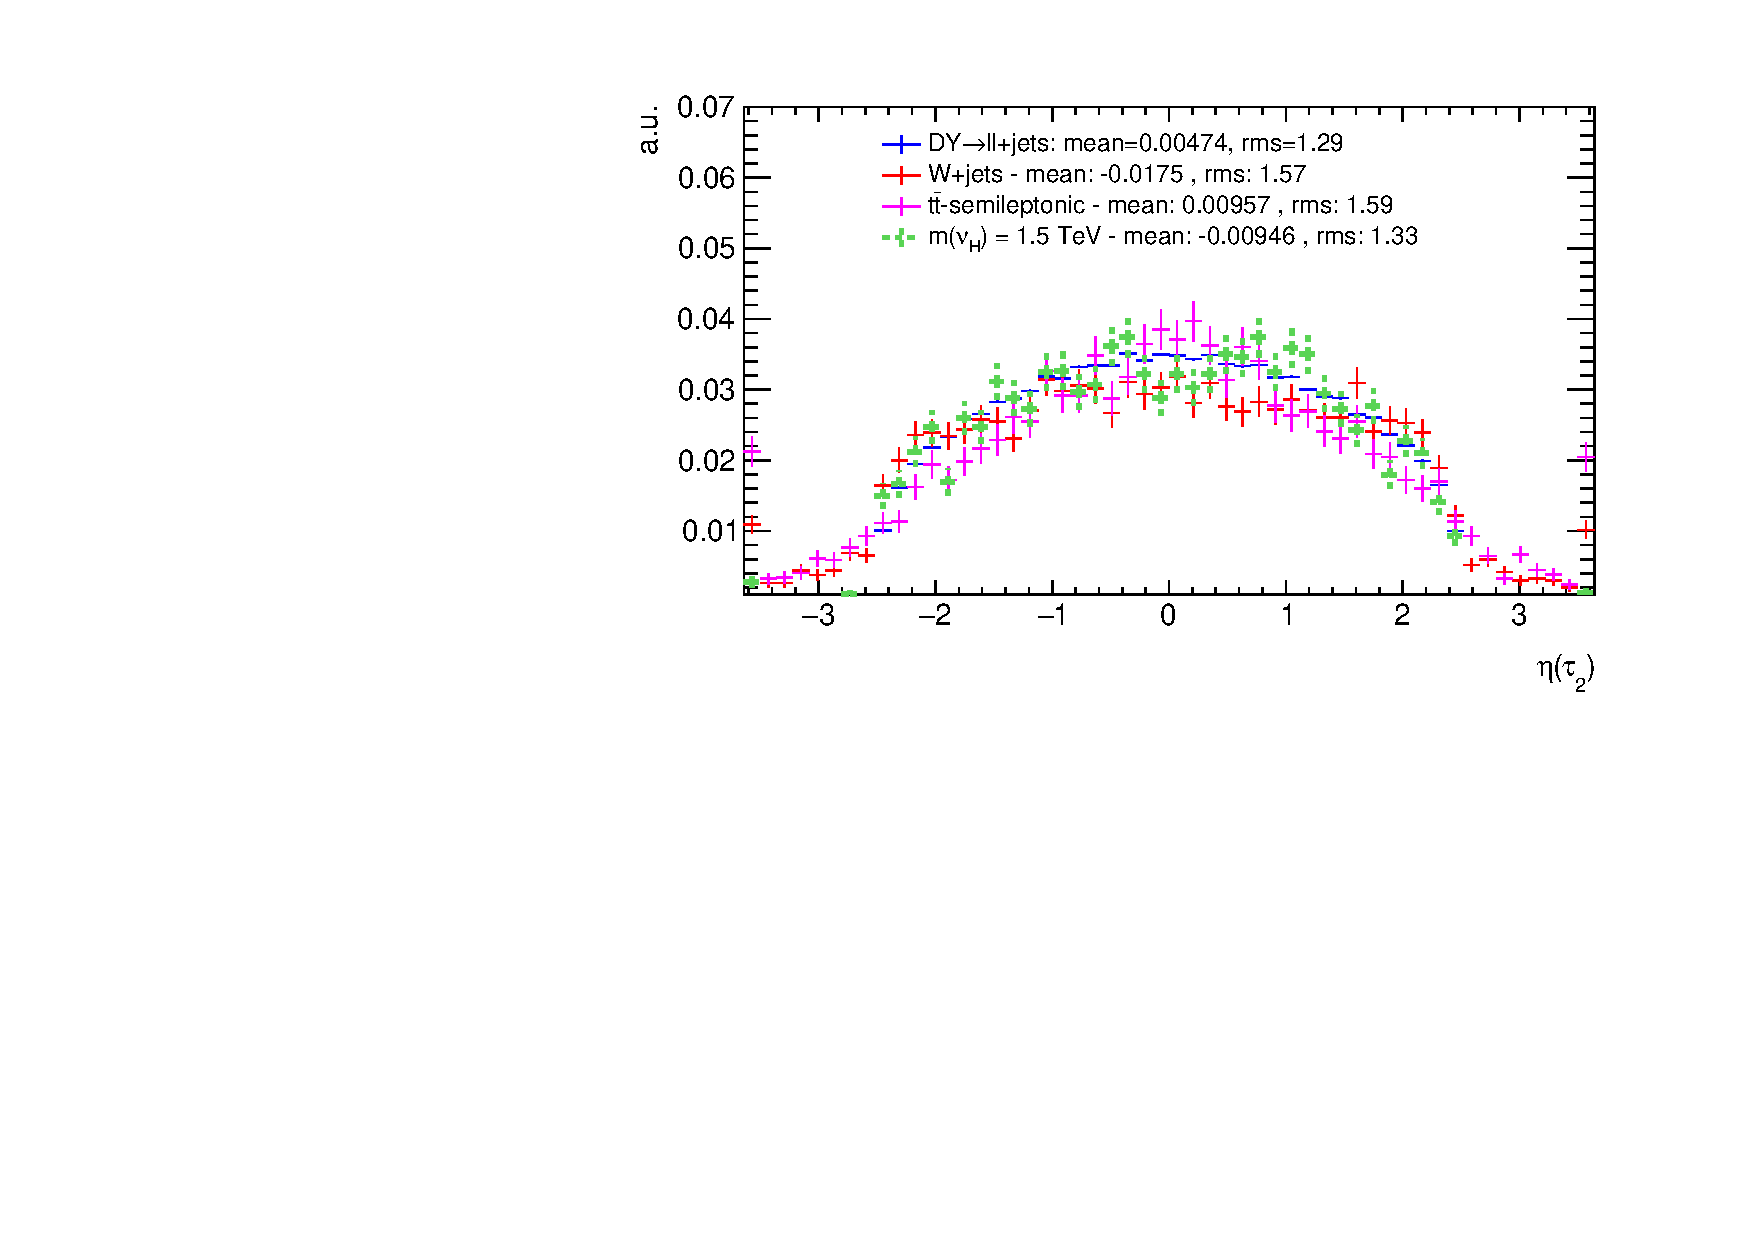
\includegraphics[width=\linewidth]{Plots/tau2_eta_unitNC.pdf}
\caption{Unit plot of $\eta$ from the sub-leading $\tau$ with no cuts}
\label{fig: tau2etaunitNC}
\end{figure}

\begin{figure}
\centering
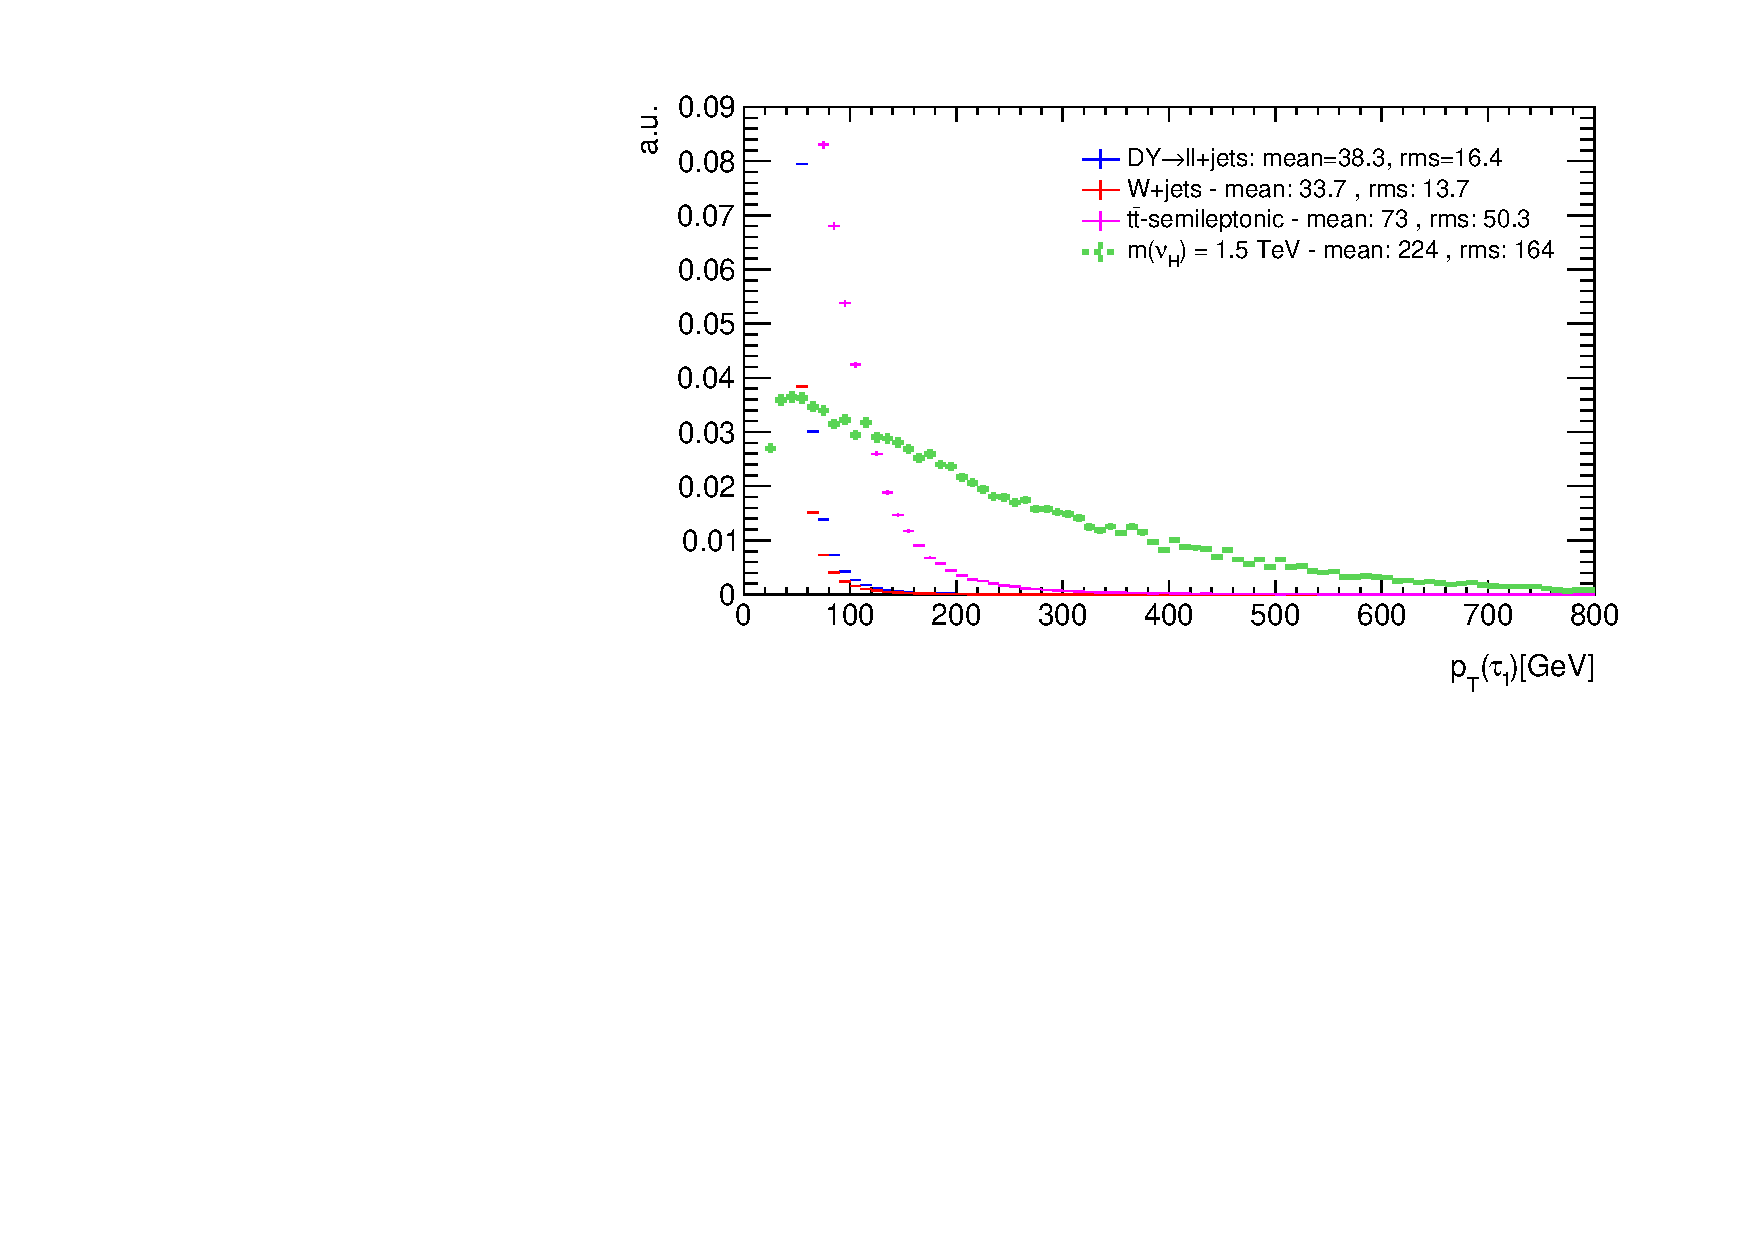
\includegraphics[width=\linewidth]{Plots/tau1_pt_unitNC.pdf}
\caption{Unit plot of $p_{T}$ of leading $\tau$ with no cuts}
\label{fig: tau1ptunitNC}
\end{figure}

To understand the definition of $H_{T}$ and $S_{T}$ mentioned in Chapter \ref{sec:definitions}, the plots in Figure \ref{fig: ptUnitPlots} are shown. The four plots show a separation, in some cases a smaller than others, between the signal and backgrounds distributions. A tendency of the signal jets to have greater transverse momentum than the ones in the backgrounds is shown. This tendency is also displayed for both $\tau$'s. Hence, the distributions of $H_{T}$ and $S_{T}$ should show a similar behaviour because this variables are the result of adding the transverse momentum of jets and $\tau$'s in the event.

\begin{figure}       
        \centering
        \begin{subfigure}[b]{0.475\textwidth}
            \centering
            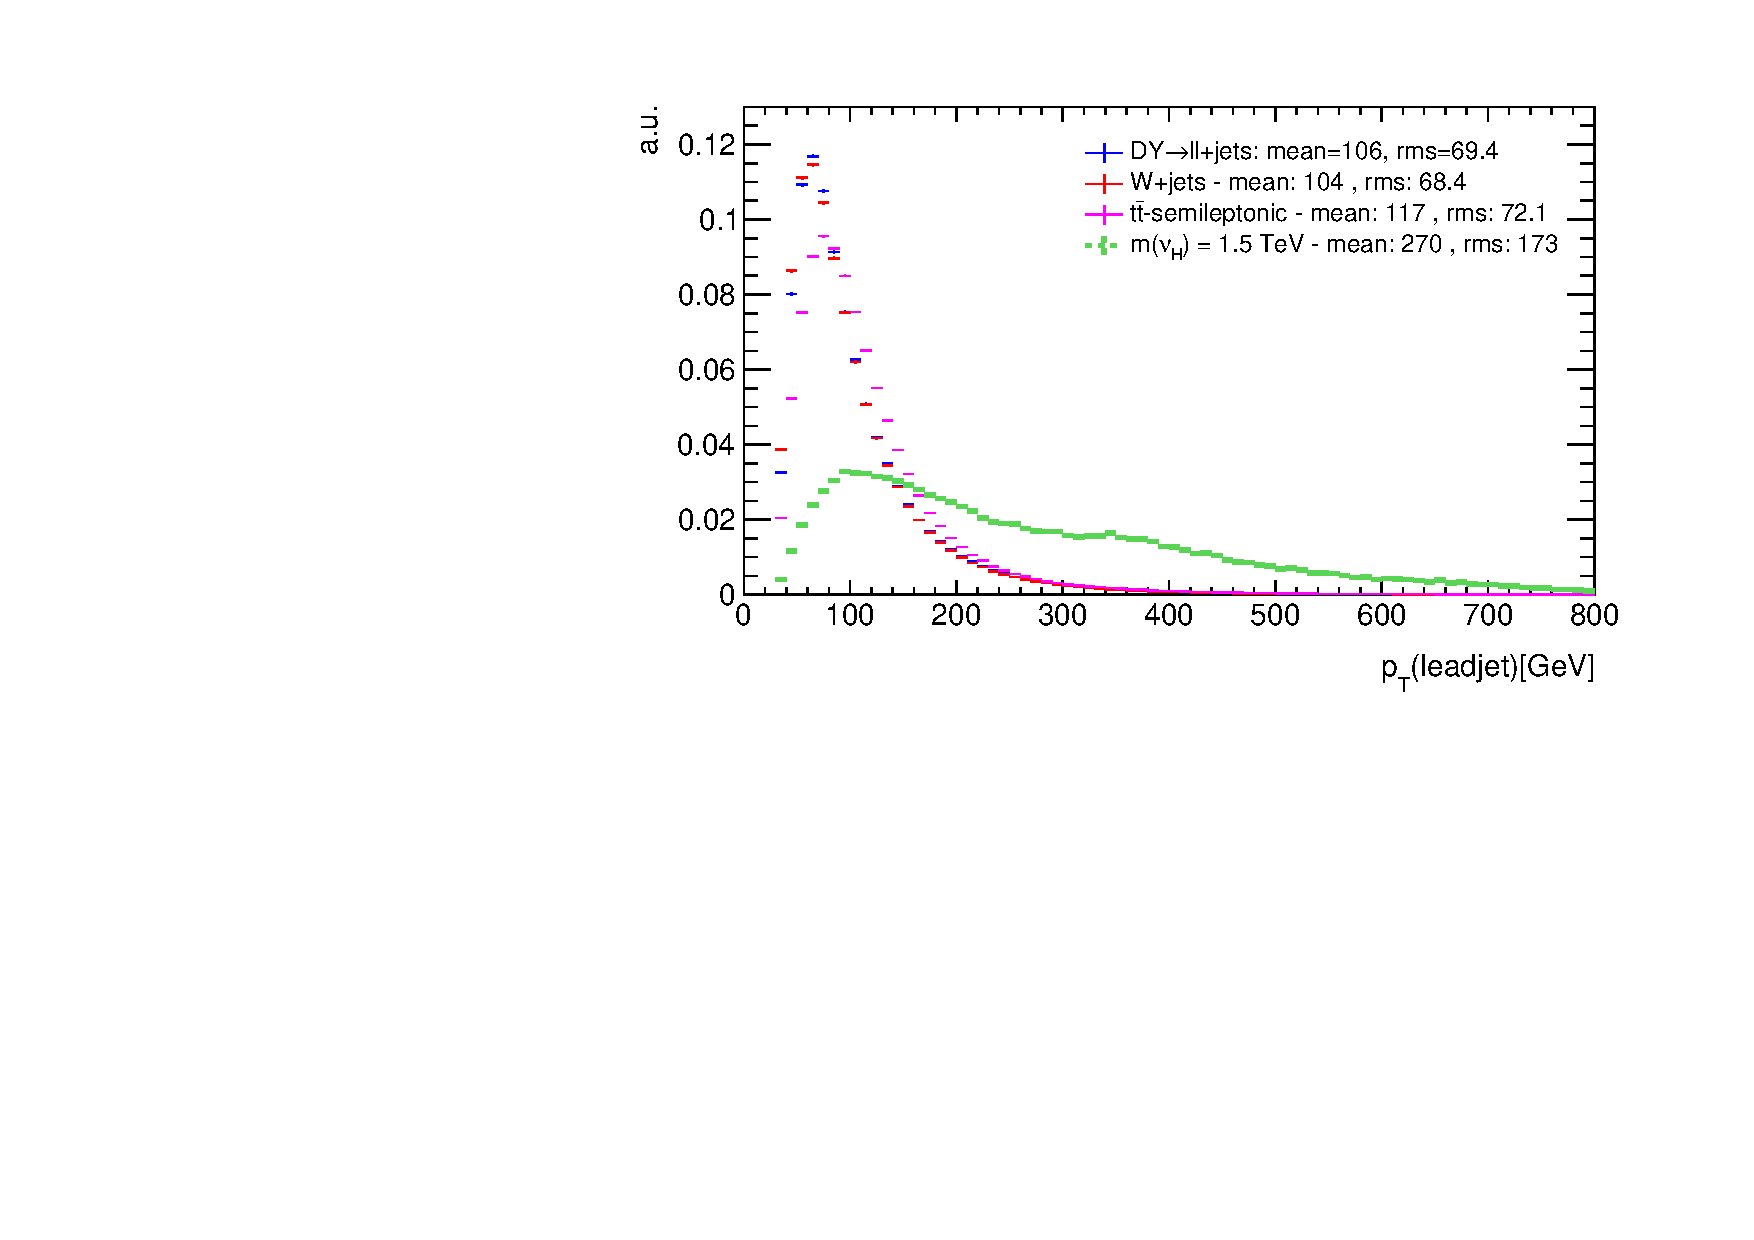
\includegraphics[width=\textwidth]{Plots/ljet_pt_unitNC}
            \caption[]%
            {{\small Leading jet $p_{T}$ unit plot}}    
            %\label{fig:mean and std of net14}
        \end{subfigure}
        \hfill
        \begin{subfigure}[b]{0.475\textwidth}  
            \centering 
            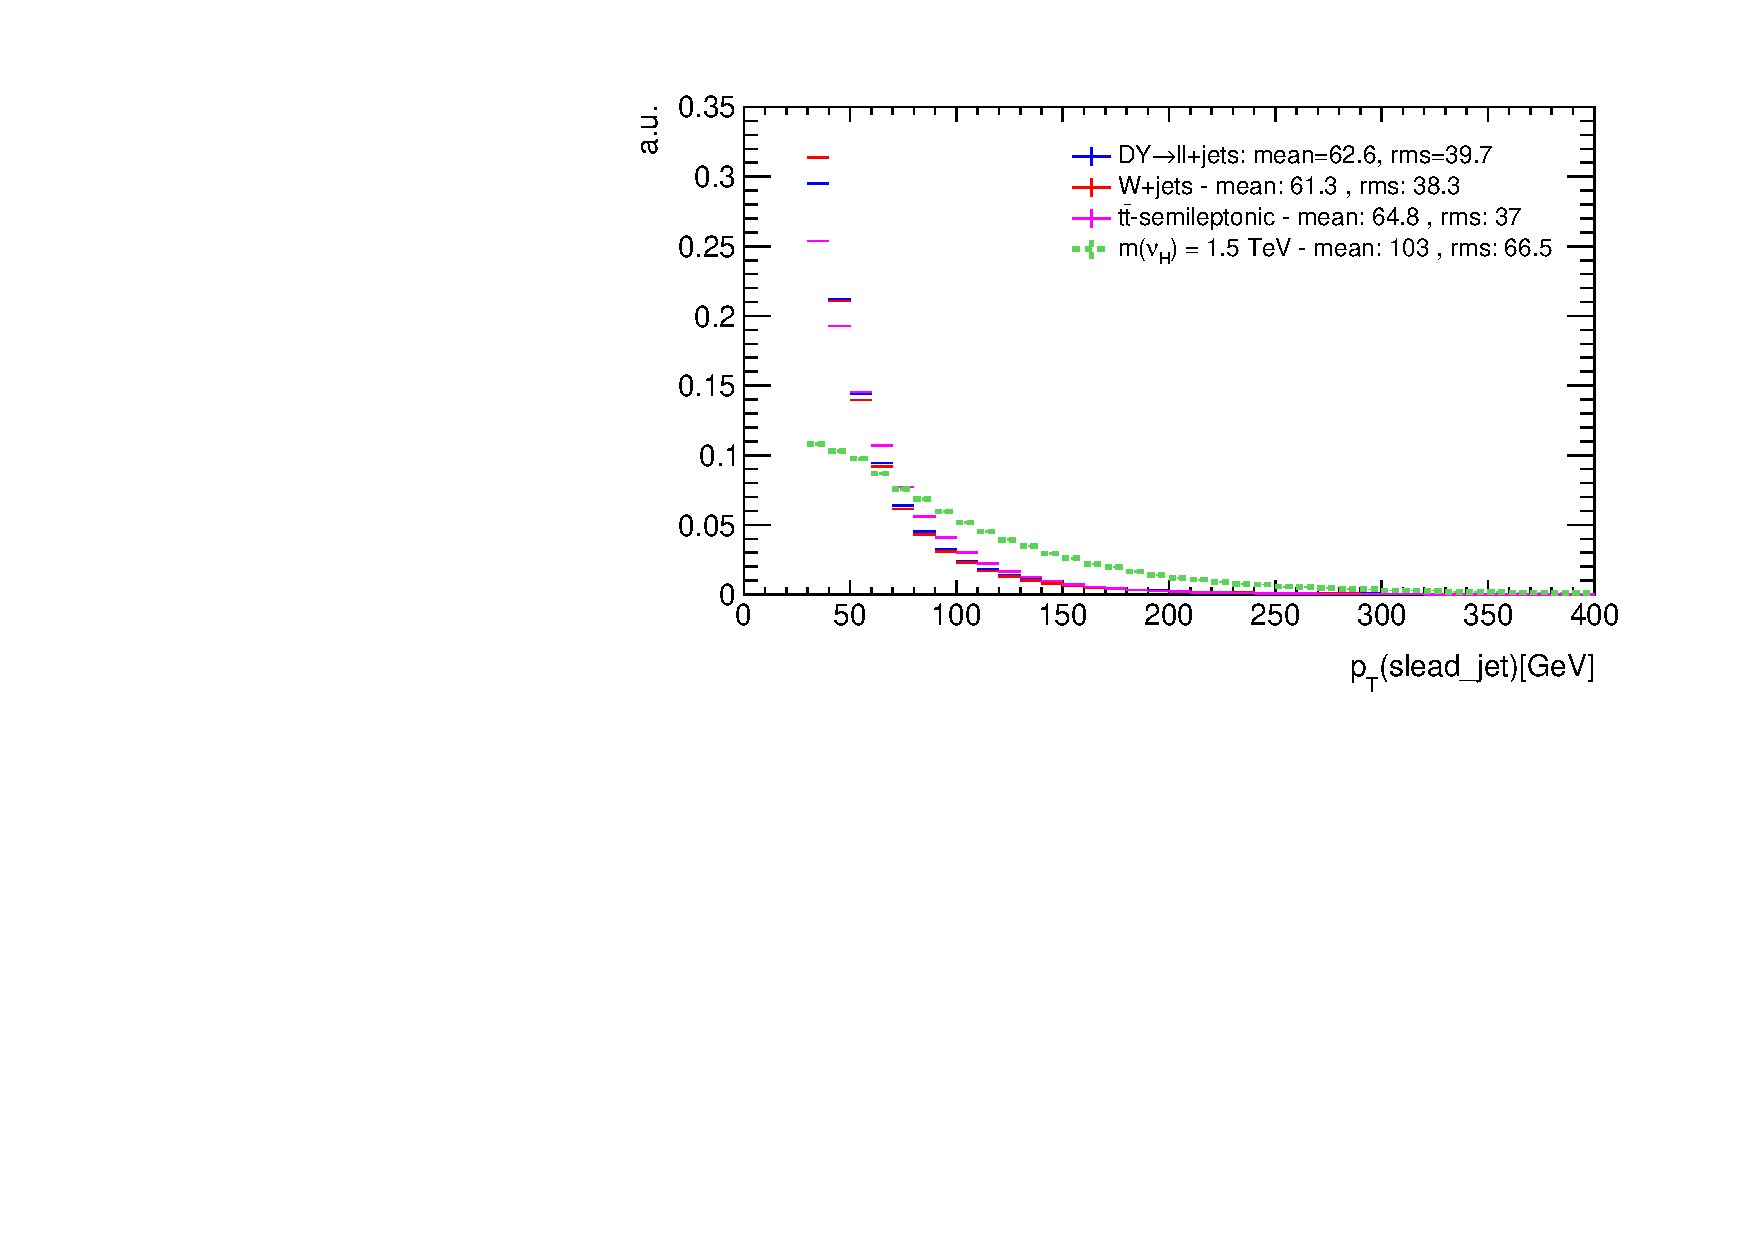
\includegraphics[width=\textwidth]{Plots/sjet_pt_unitNC}
            \caption[]%
            {{\small Sub-leading jet $p_{T}$ unit plot}}    
            %\label{fig:mean and std of net24}
        \end{subfigure}
        \vskip\baselineskip
        \begin{subfigure}[b]{0.475\textwidth}   
            \centering 
            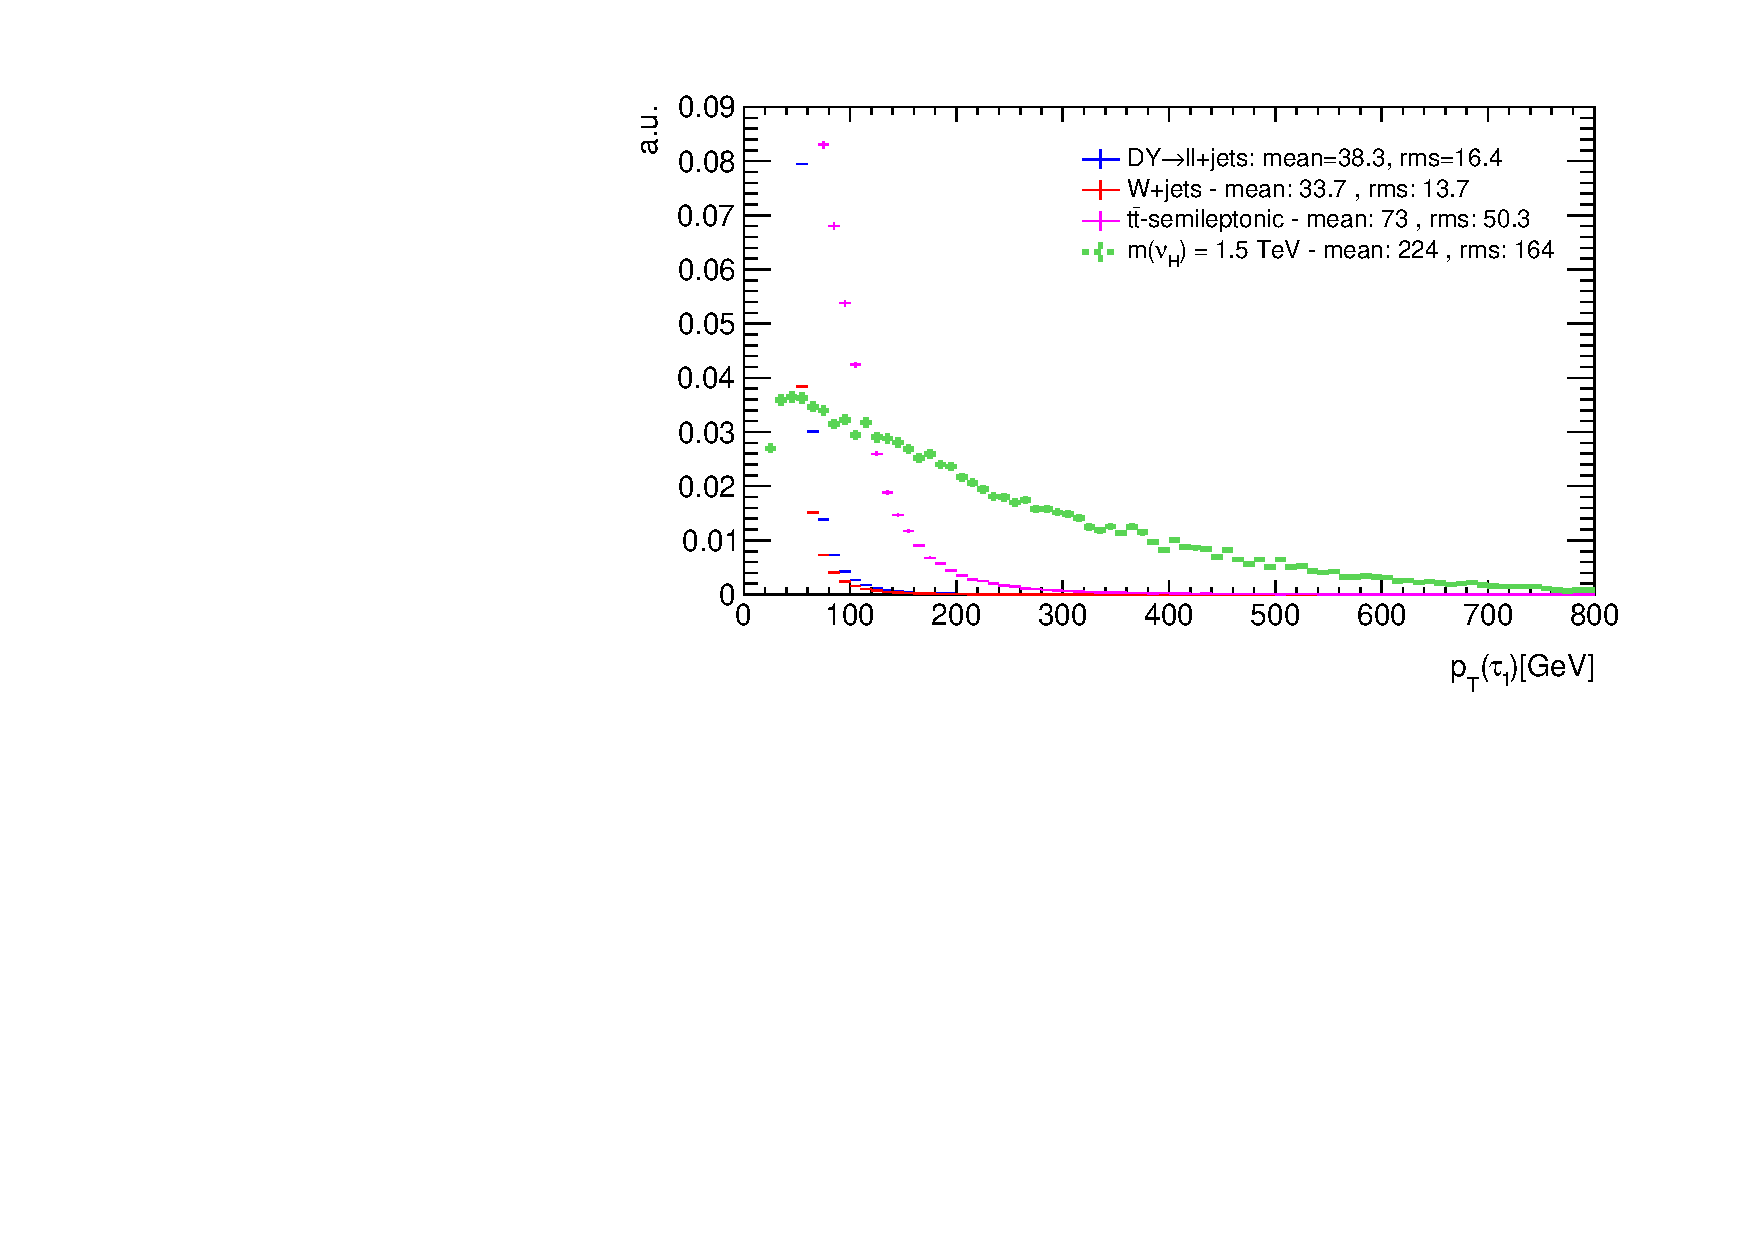
\includegraphics[width=\textwidth]{Plots/tau1_pt_unitNC}
            \caption[]%
            {{\small Leading $\tau$ $p_{T}$ unit plot}}    
            %\label{fig:mean and std of net34}
        \end{subfigure}
        \quad
        \begin{subfigure}[b]{0.475\textwidth}   
            \centering 
            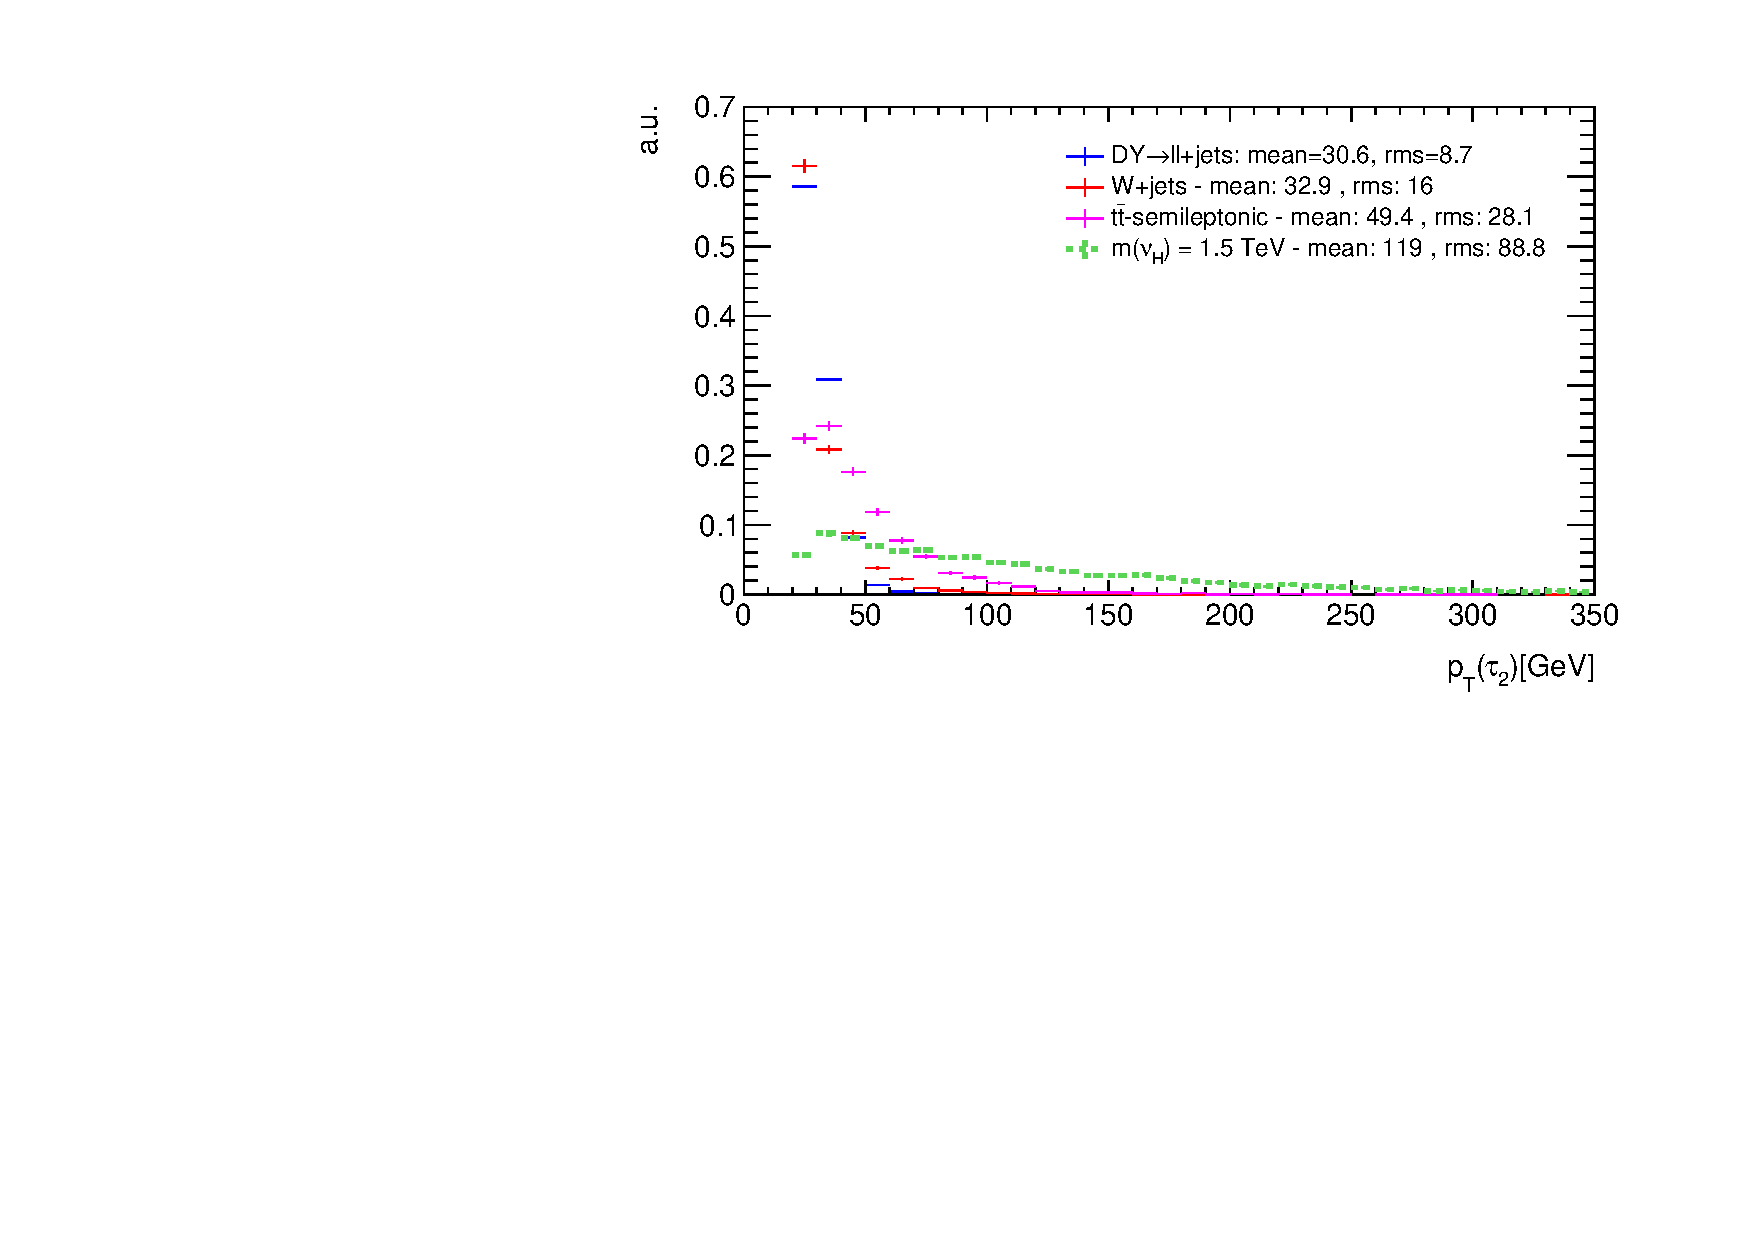
\includegraphics[width=\textwidth]{Plots/tau2_pt_unitNC}
            \caption[]%
            {{\small Sub-leading $\tau$ $p_{T}$ unit plot}}    
            %\label{fig:mean and std of net44}
        \end{subfigure}
        \caption[ $p_T$ unit plots for different bodies in the event]
        {\small $p_T$ unit plots for different bodies in the event} 
         \label{fig: ptUnitPlots}
\end{figure}

In Figures \ref{fig: HTunitNC} and \ref{fig: STunitNC}, the normalized plots with no cuts of $H_{T}$ and $S_{T}$ are shown. It can be seen that indeed a greater separation between signal and background was achieved. Unlike the distributions of the $\tau$'s and jets transverse momentum, the maxima of $H_{T}$ and $S_{T}$ lie outside the backgrounds distributions. Furthermore, the background that overlaps at a greater energy with the signal corresponds to $t\bar{t}$. Taking into account what was mentioned in section \ref{sec: cutdefinitions}, the overlap between the signal and this background could be reduced with the cut related with the number of B-jets in the event. This is why this two variables need to be studied closer in the analysis.

\begin{figure}
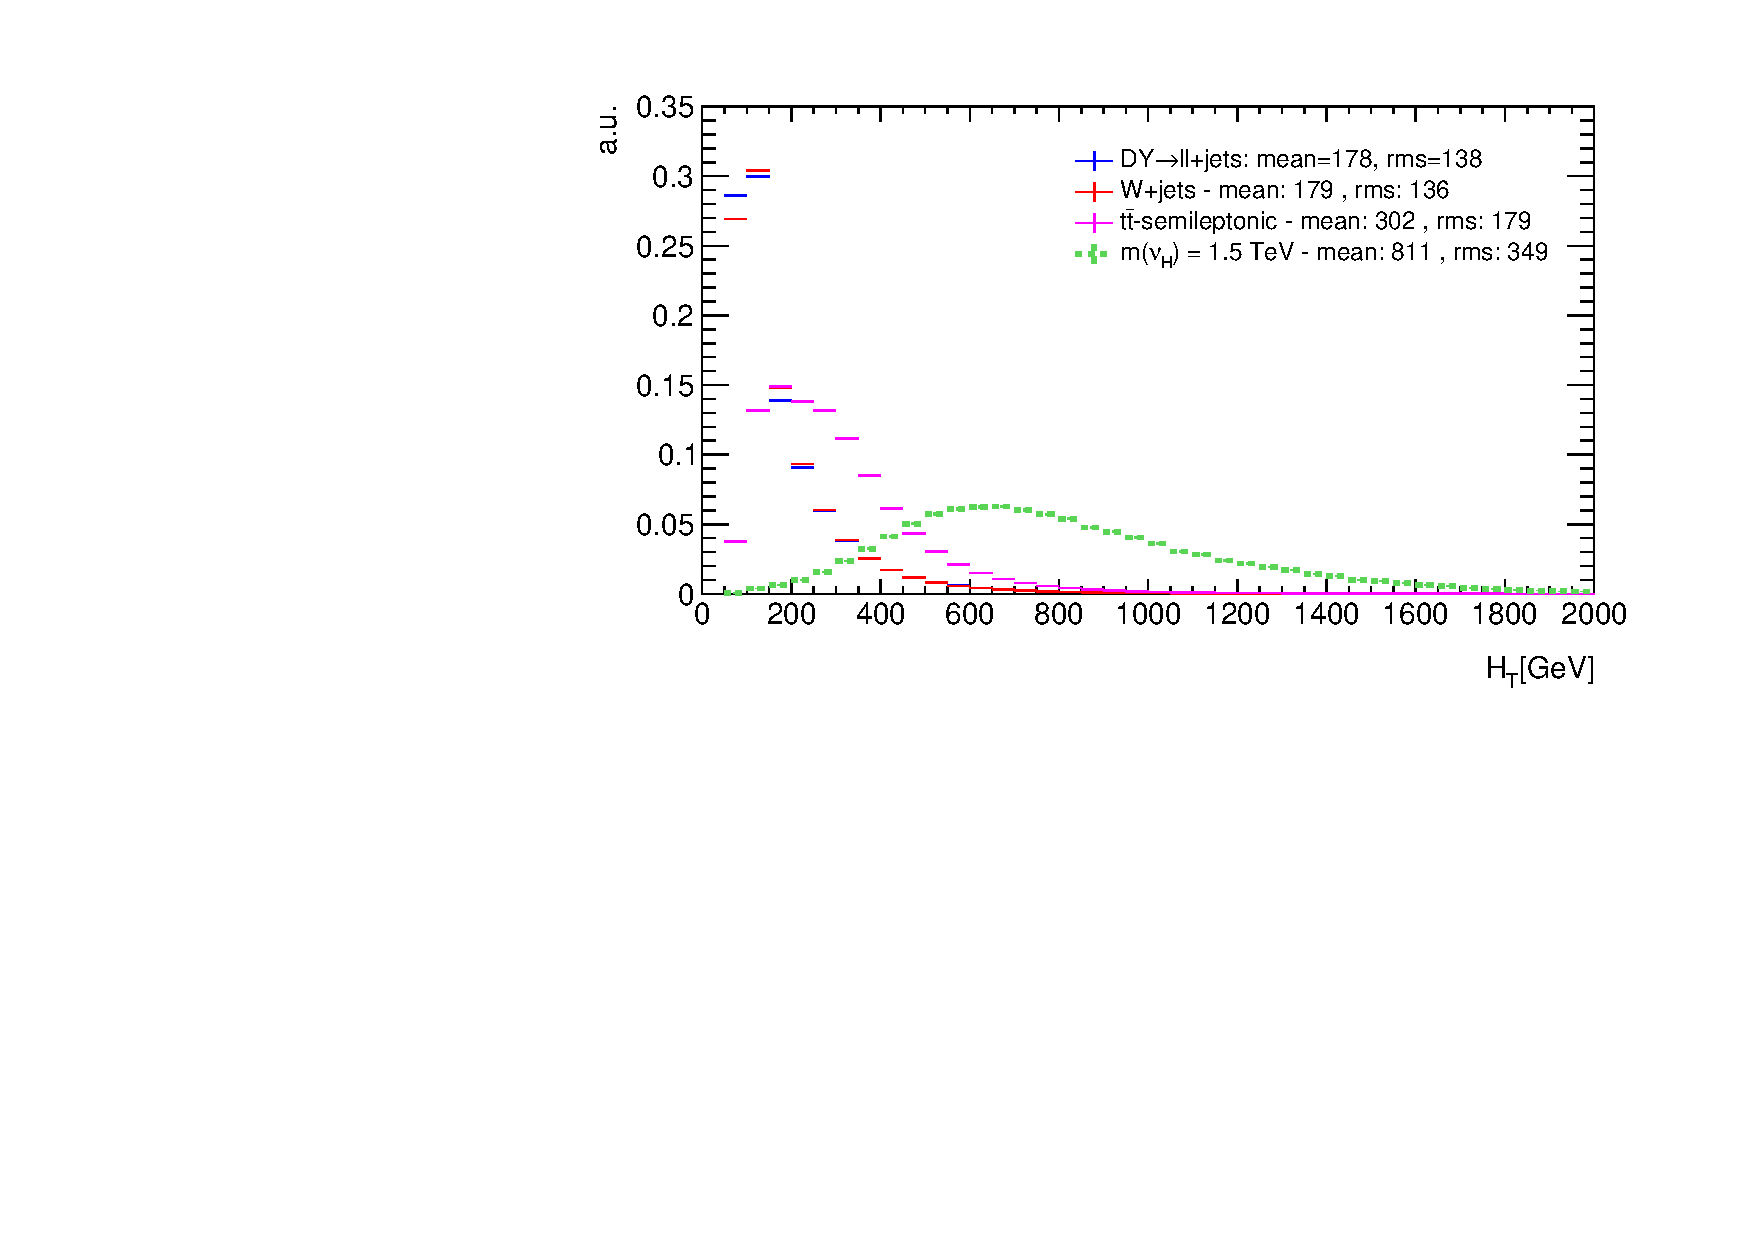
\includegraphics[width=\linewidth]{Plots/HT_unitNC.pdf}
\caption{Unit plot of $H_{T}$ with no cuts}
\label{fig: HTunitNC}
\end{figure}

\begin{figure}
\centering
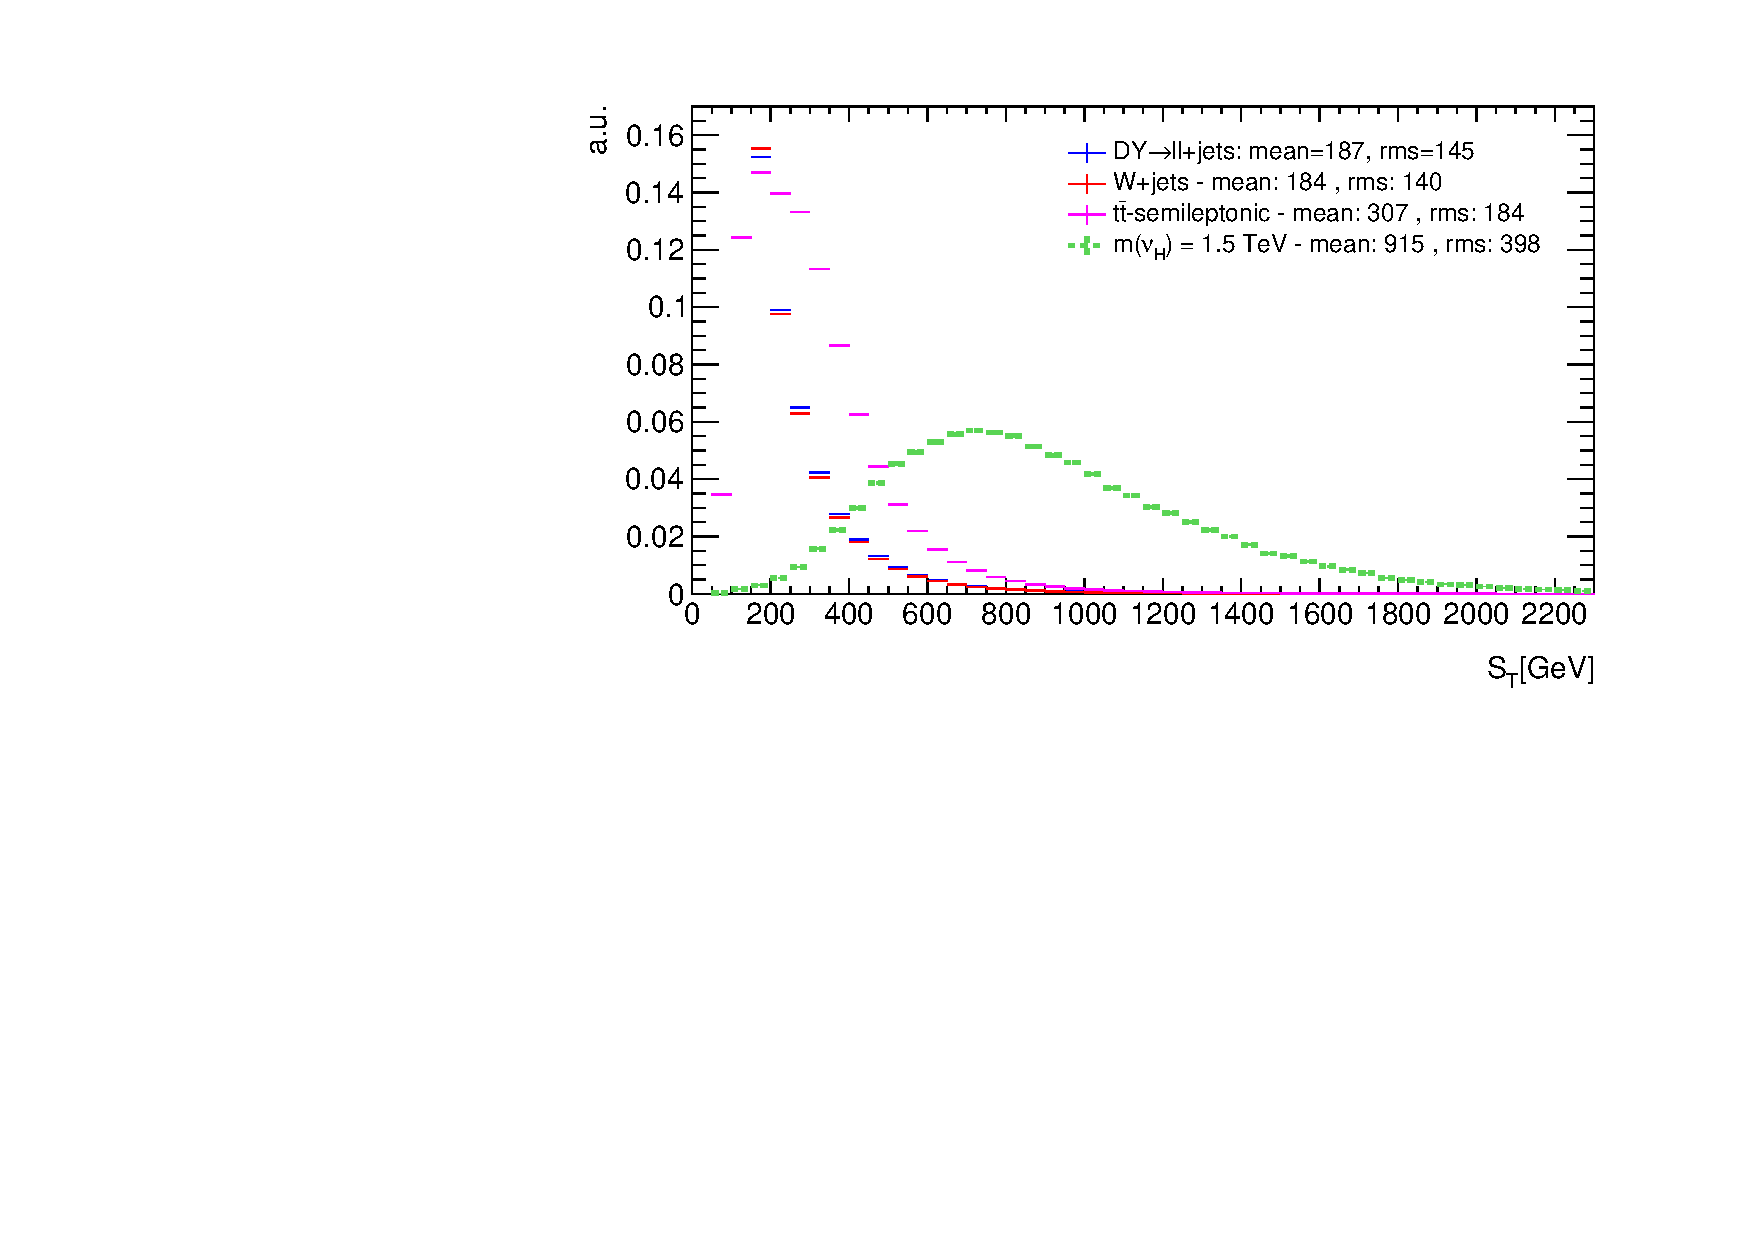
\includegraphics[width=\linewidth]{Plots/ST_unitNC.pdf}
\caption{Unit plot of $S_{T}$ with no cuts}
\label{fig: STunitNC}
\end{figure}

Another variable relevant for the analysis was found out to be $m(jj)$. The reason for a further analysis of this variable is shown in Figure \ref{fig: mjjUnitNC}. As in the case of $H_{T}$ and $S_{T}$, the distribution of the mass of the Di-Jet Pair shows a separation between the signal and the three backgrounds. Furthermore, it shows a greater separation than the one observed for both $H_{T}$ and $S_{T}$. That is why, the variable $m(jj)$, or the total mass of the Di-Jet Pair, has to be studied more closely, because it shows potential for a separation between signal and backgrounds.

\begin{figure}
\centering
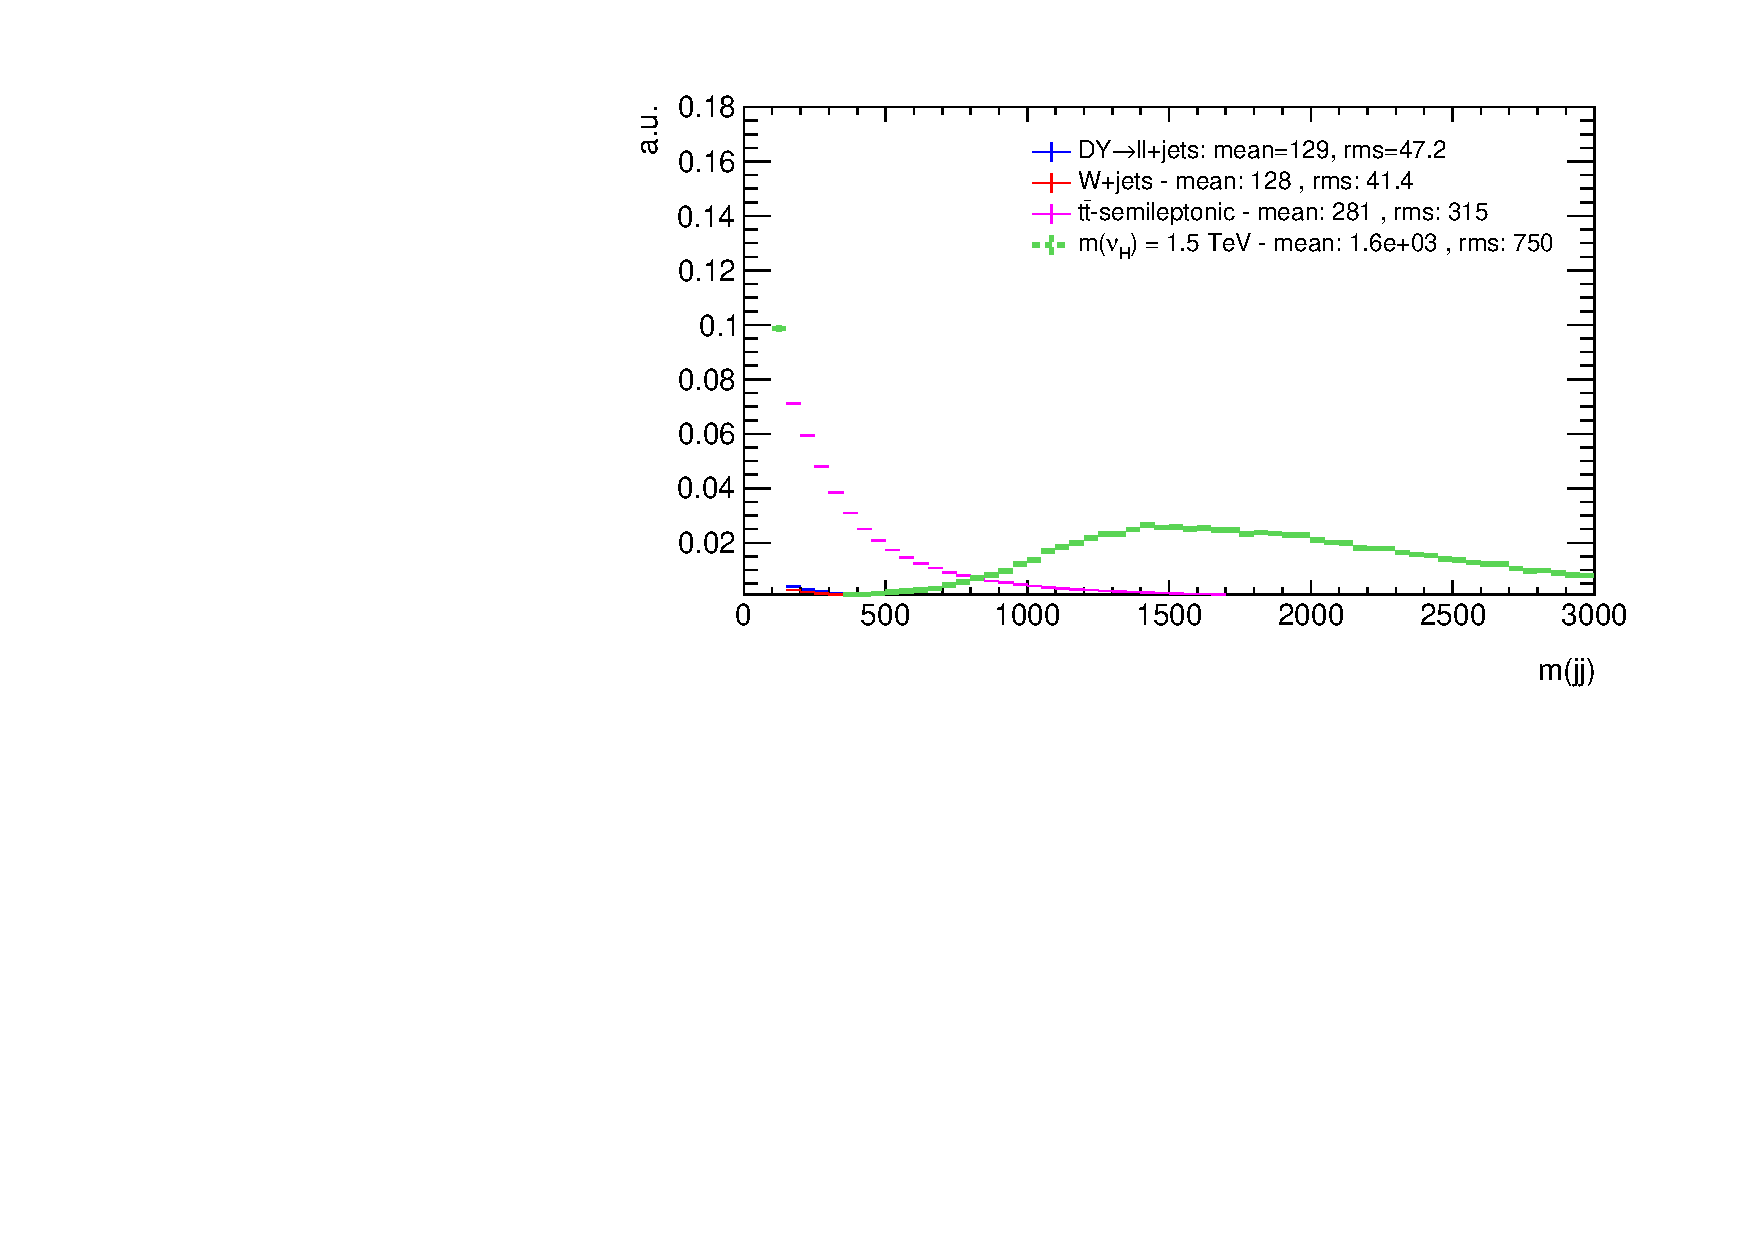
\includegraphics[width=\linewidth]{Plots/mjj_unitNC.pdf}
\caption{Unit plot of $m(jj)$ with no cuts}
\label{fig: mjjUnitNC}
\end{figure}

In Figures \ref{fig: HTunitVBF} and \ref{fig: STunitVBF}, the plots incuding cuts of $H_{T}$ and $S_{T}$ respectively are shown. Both plots include all the cuts mentioned in section \ref{sec: selectionCriteria}. A rebining of the histograms was necessary, because due to the cuts, the number of backgrounds events decreased significantly. This made the error bars for these histograms larger making the analysis of the plot more difficult. For that reason, a bin size of 400 GeV was defined for both of these plots. Comparing the two signal histograms, it can be seen that the maximum of the $H_{T}$ distribution still overlaps with the background distributions. Although the signal in this case appears on top of the background, it has to be noted that this normalized plots are only useful to get an idea of the distribution shapes. That is why the fact the the signal appears on top of the background does not mean that the signal can be detected over the background for this value. On the contrary, the maximum of the $S_{T}$ signal distribution has its maximum when the background distributions start to decay. This distribution shape  difference between $H_{T}$ and $S_{T}$ is related with the fact that the signal has $\tau$'s with higher $p_{T}$ than the ones found in the backgrounds.

\begin{figure}
\begin{center}
 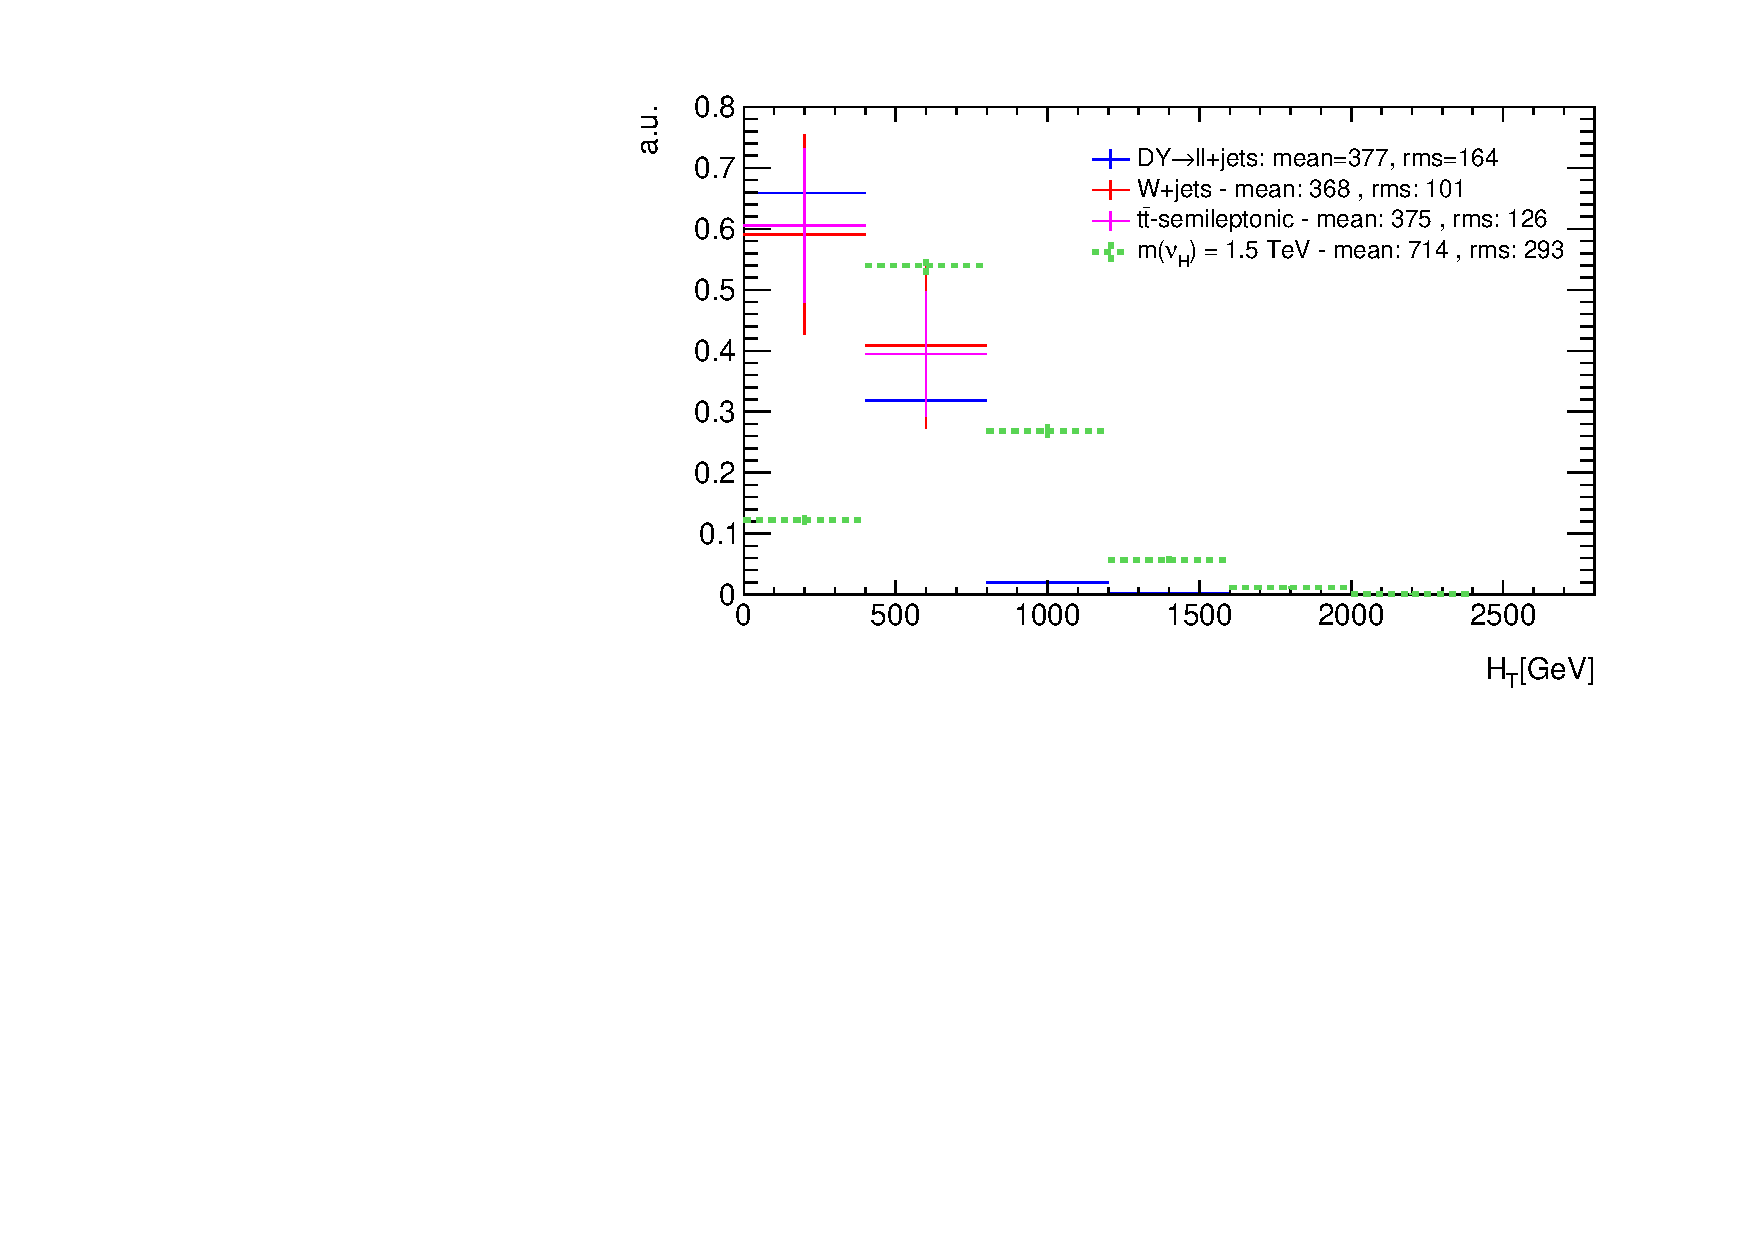
\includegraphics[width=\linewidth]{Plots/HT_unitVBF.pdf}
\end{center}
\caption{Unit plot of $H_{T}$ with VBF cuts}
\label{fig: HTunitVBF}
\end{figure}

\begin{figure}
\centering
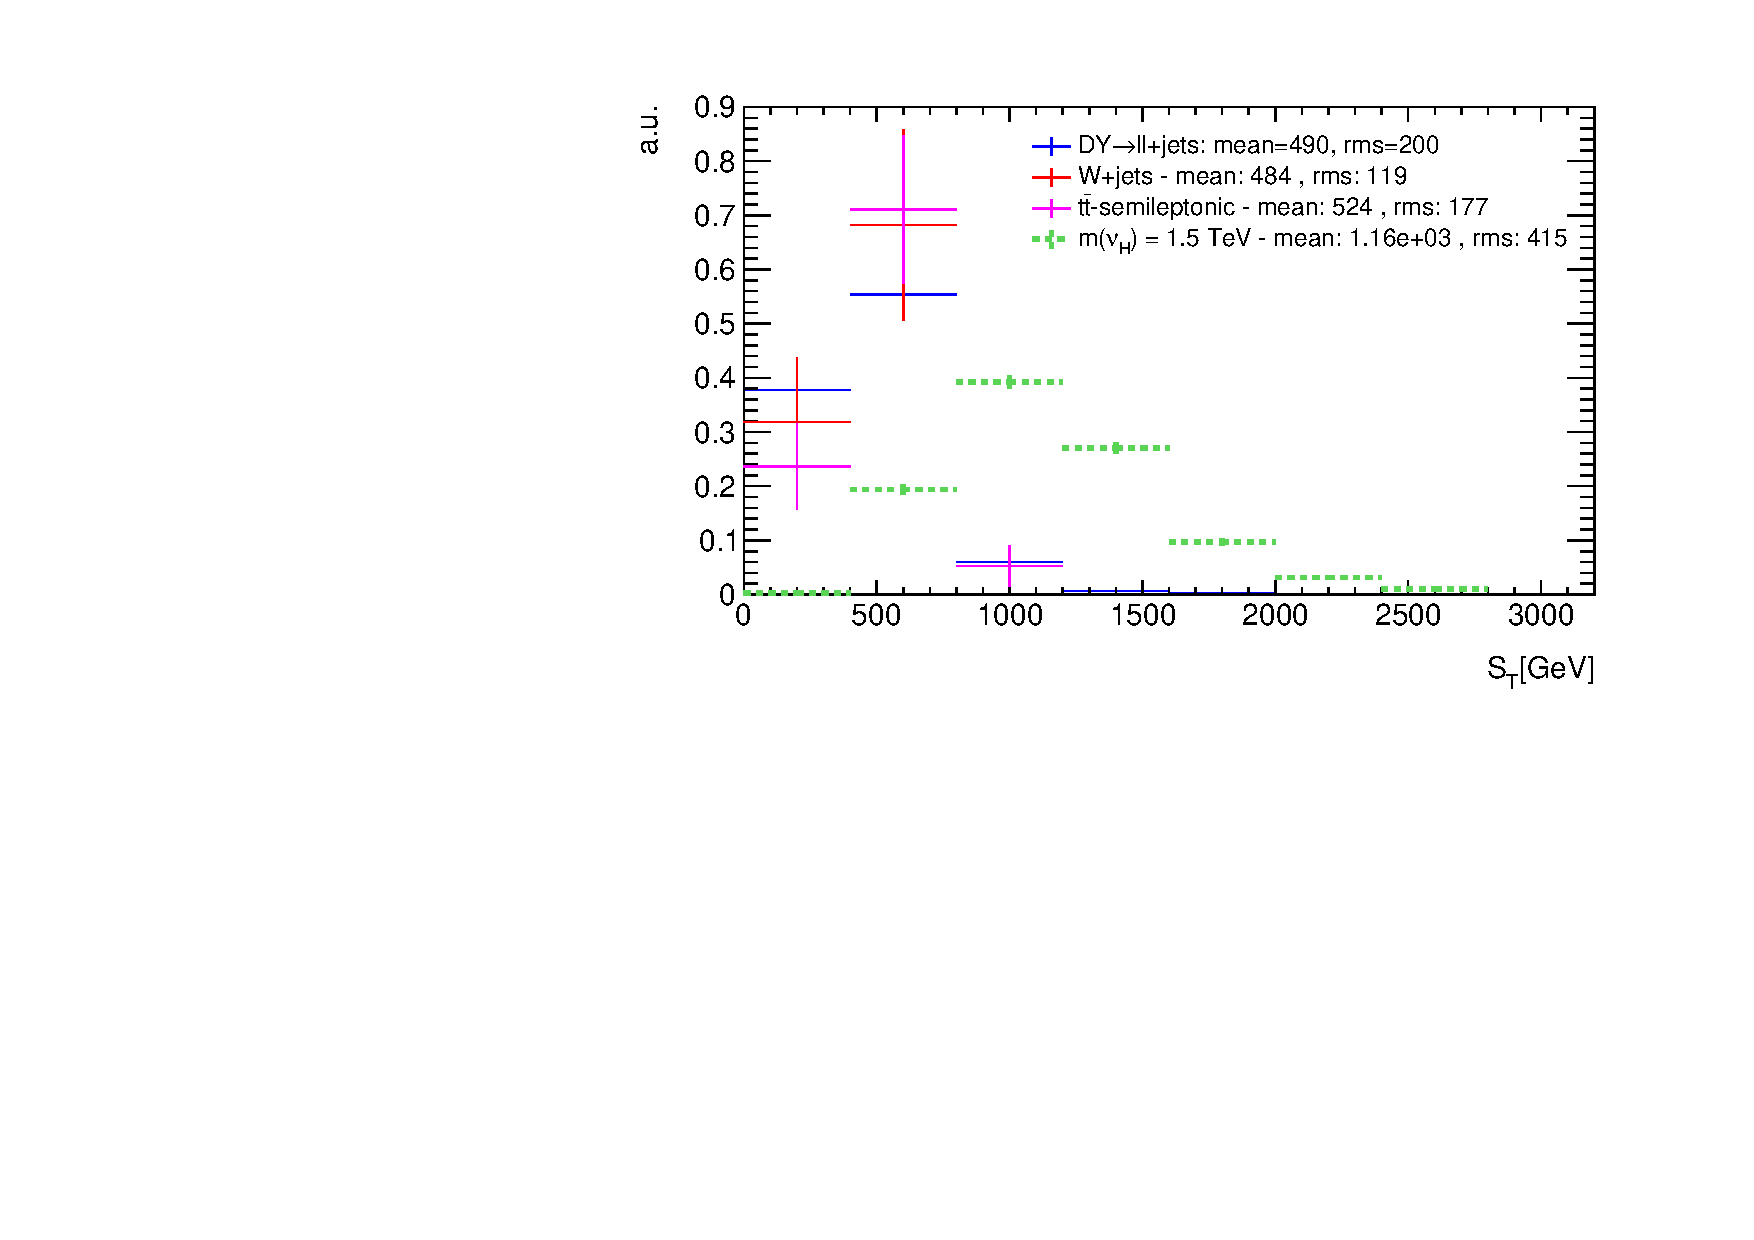
\includegraphics[width=\linewidth]{Plots/ST_unitVBF.pdf}
\caption{Unit plot of $S_{T}$ with VBF cuts}
\label{fig: STunitVBF}
\end{figure}

The mean values for $S_{T}$ shown in Figures \ref{fig: STunitNC} and \ref{fig: STunitVBF} are 915 GeV and 1160 GeV respectively. From the Feynman diagram in Figure \ref{fig: hnGamma}, it can be seen that the jets in the event and one of the taus come from the heavy neutrino decay. Taking into account that the defined mass for the heavy neutrino is 1.5 TeV, it is expected that the maximum of the $S_{T}$ distribution is around this value. This analysis leads to the conclusion that the cuts made to the histograms are helping to select the significant events, because the mean $S_{T}$ is closer to the expected value after performing all the cuts.

\section{Stack Plots}

\begin{figure}
\centering
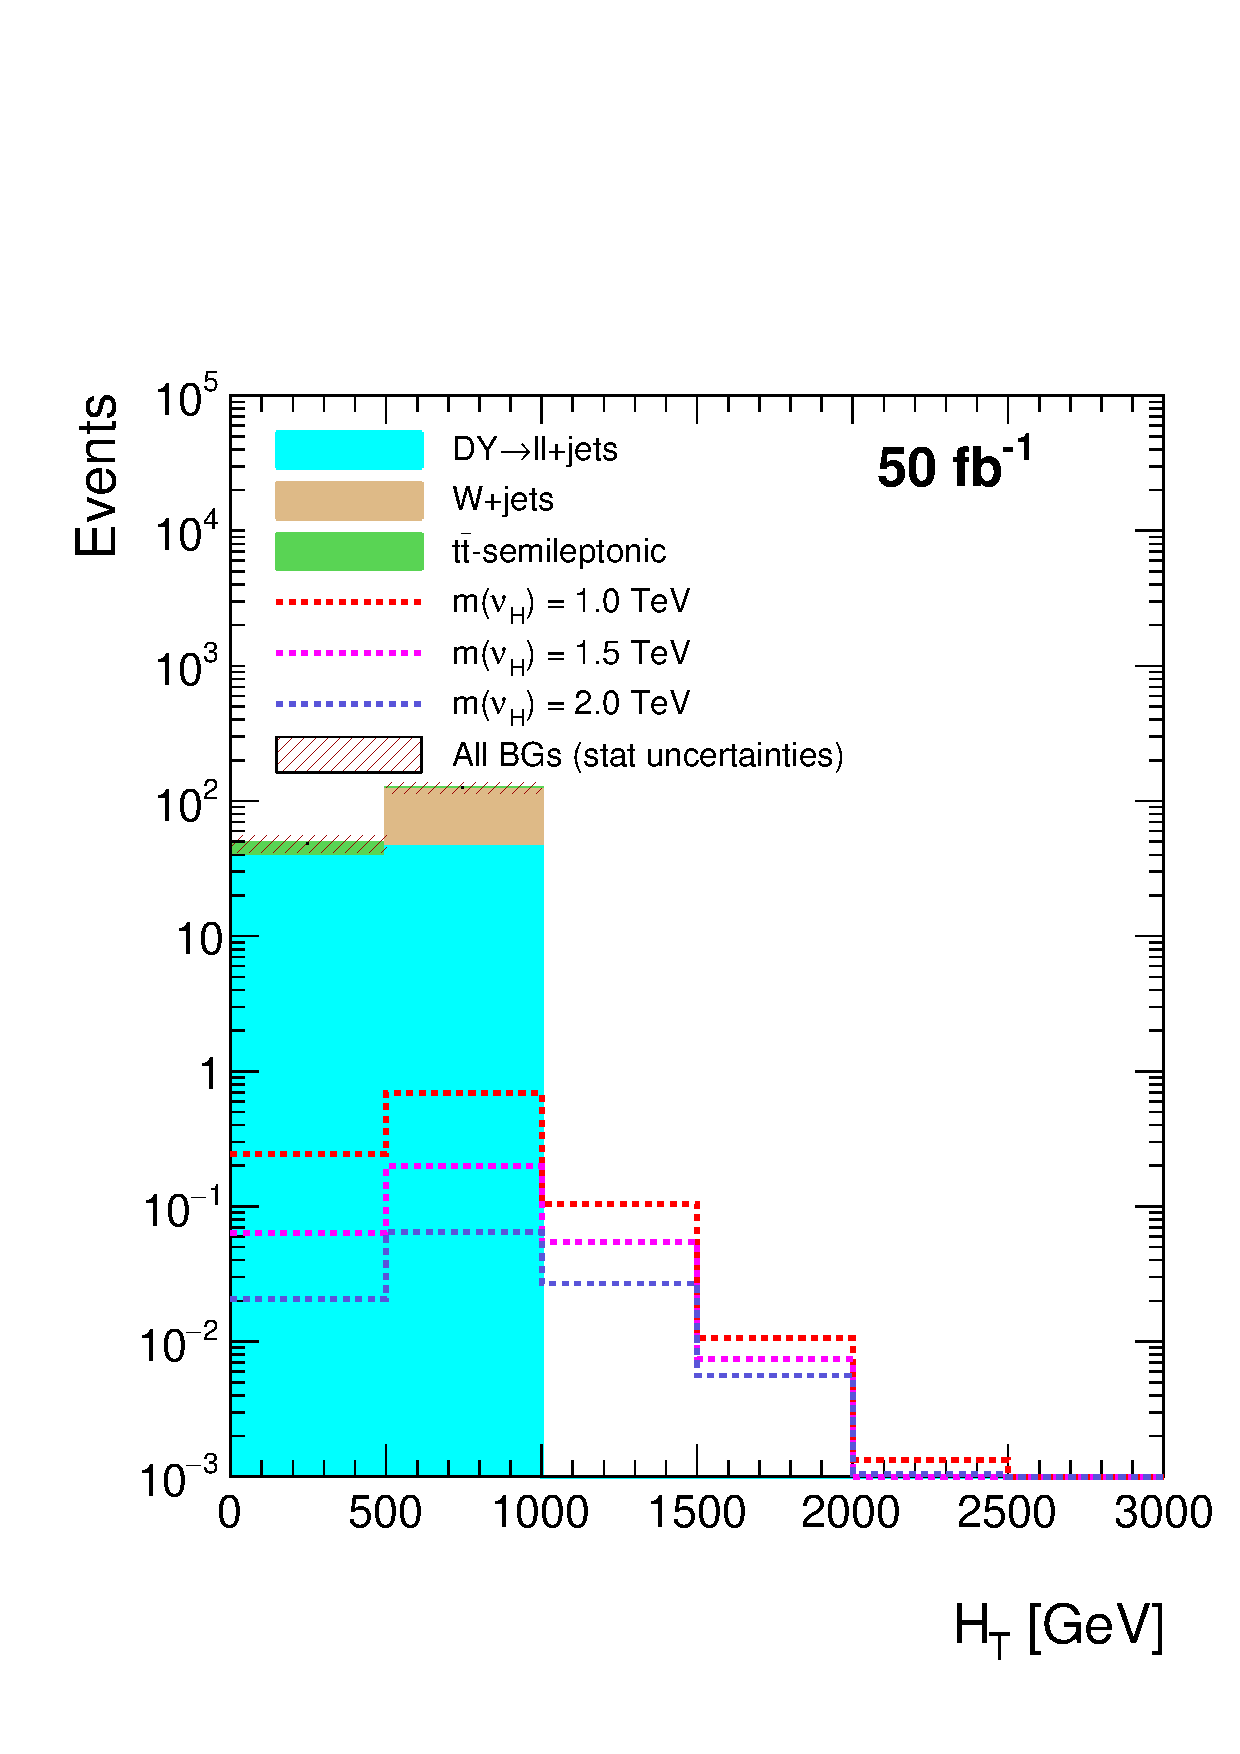
\includegraphics[width=\linewidth]{StackPlots/HT_2taus_met50_50ifb.pdf}
\caption{Stack plot of $H_{T}$ requiring two taus in the event and with $\slashed{E}_{T} > 50$}
\label{fig: HT2tausMet50}
\end{figure}

\begin{figure}
\centering
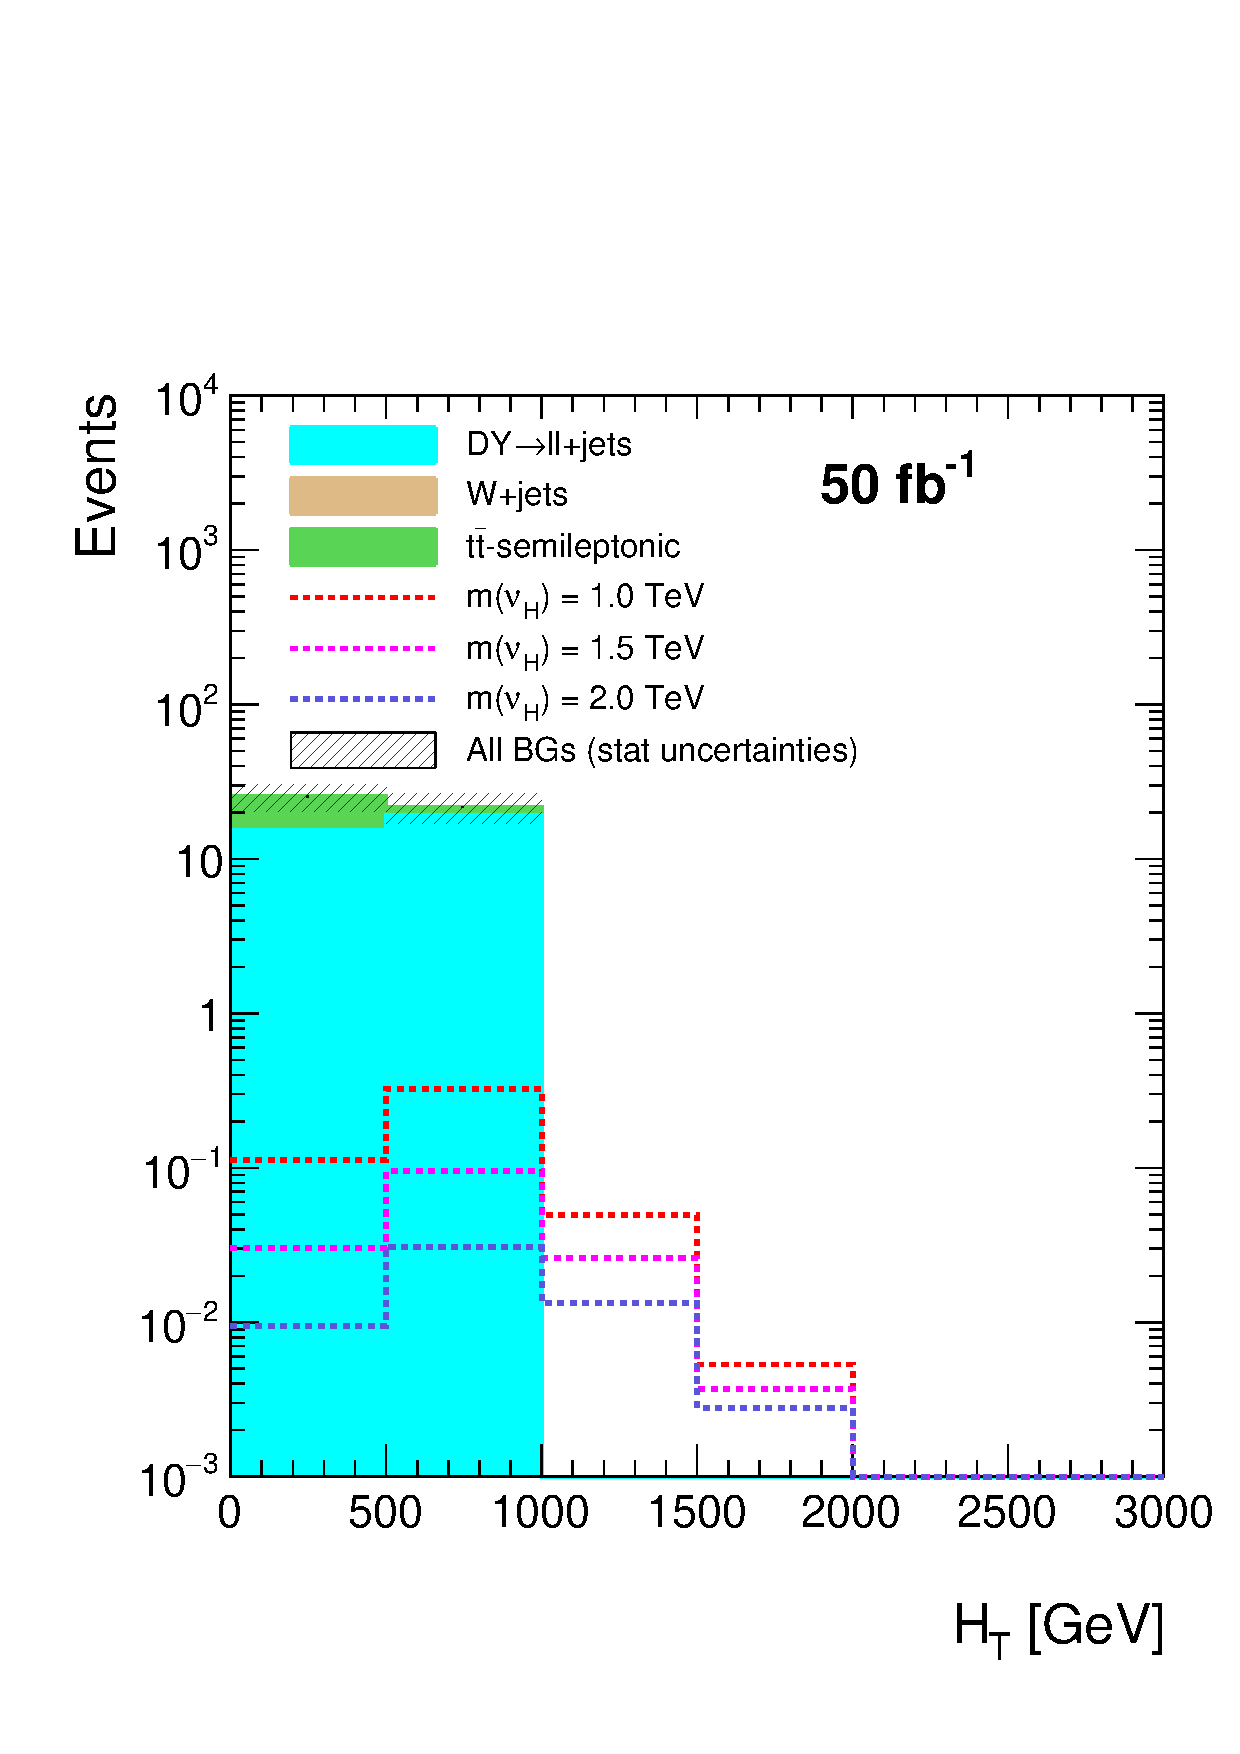
\includegraphics[width=\linewidth]{StackPlots/HT_2taus_met60_50ifb.pdf}
\caption{Stack plot of $H_{T}$ requiring two taus in the event and with $\slashed{E}_{T} > 60$}
\label{fig: HT2tausMet60}
\end{figure}

\begin{figure}
\centering
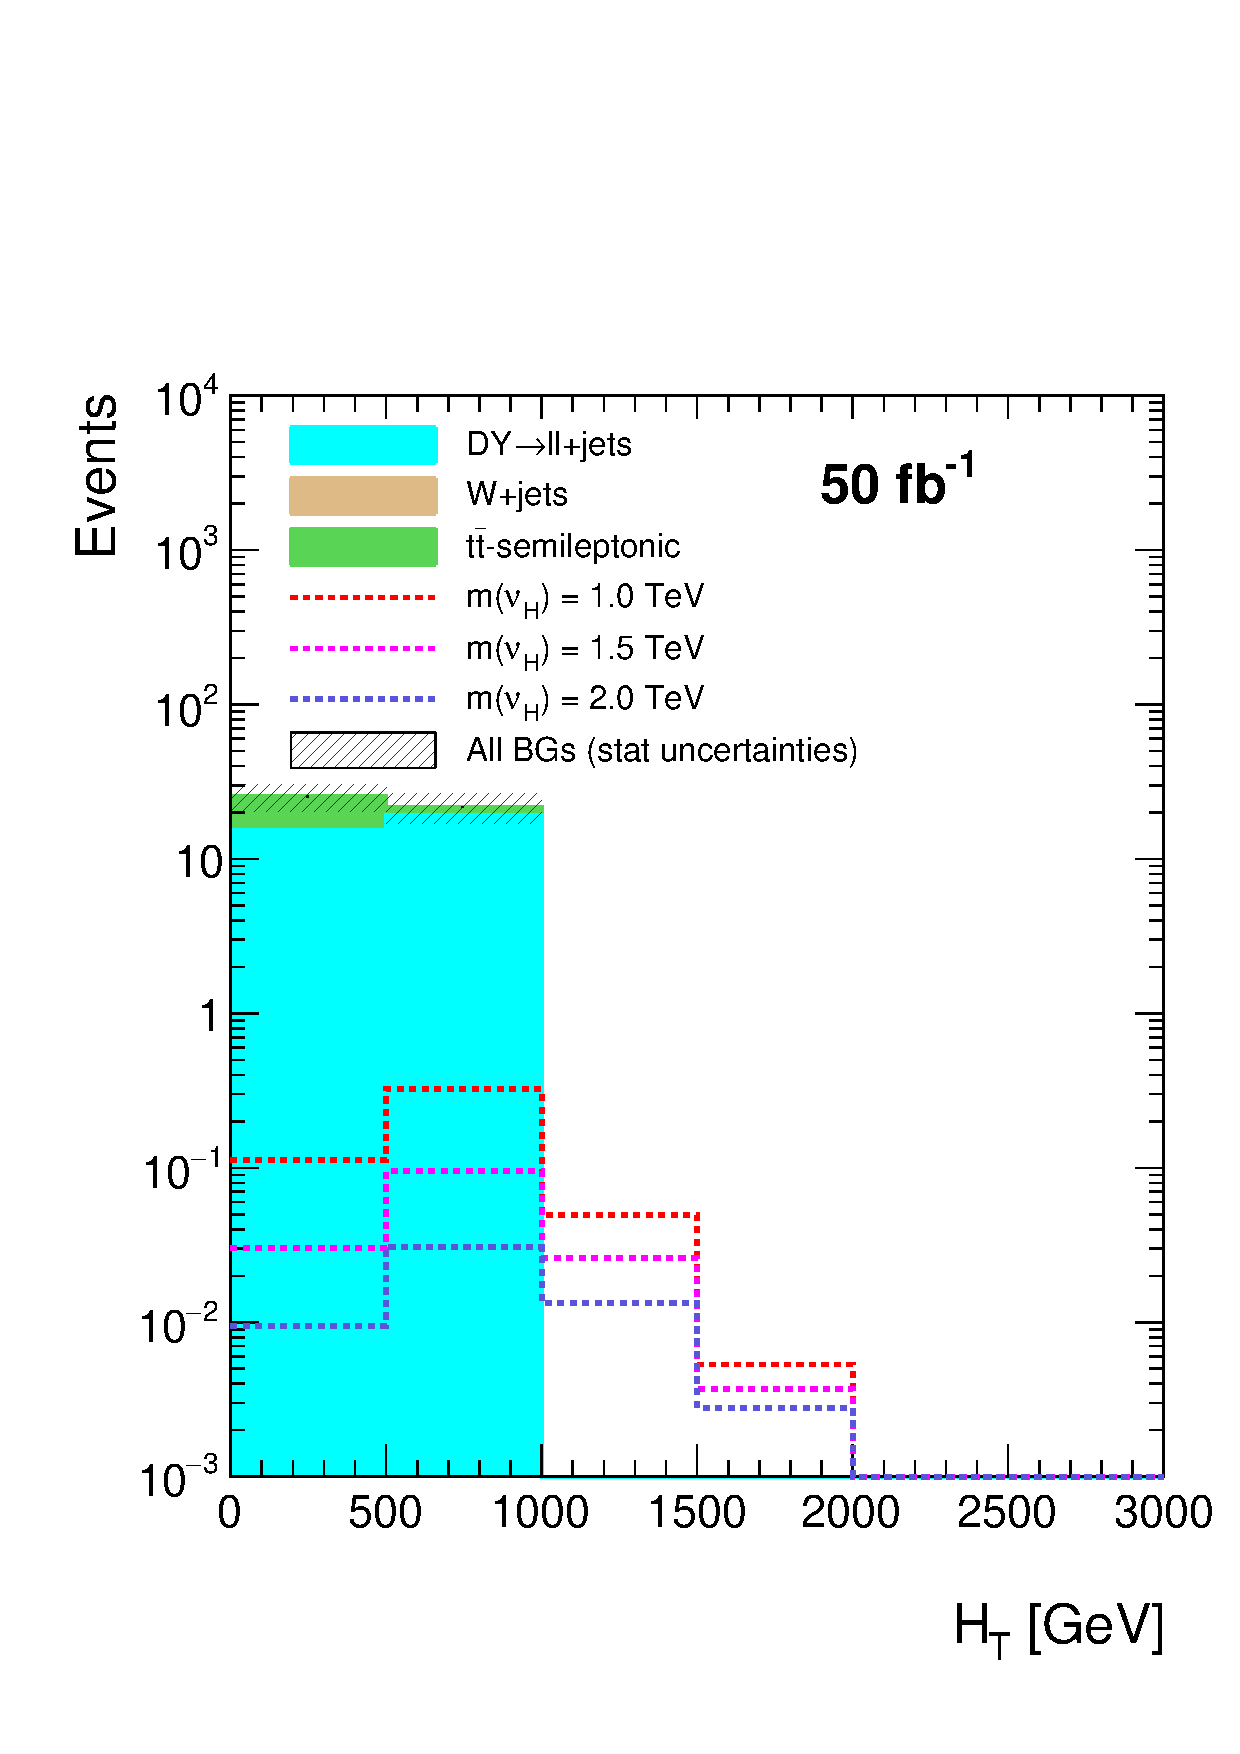
\includegraphics[width=\linewidth]{StackPlots/HT_2taus_met60_50ifb.pdf}
\caption{Stack plot of $\slashed{E_{T}}$ requiring only one tau in the event and with $\slashed{E}_{T} > 60$}
\label{fig: MET1tauMet60}
\end{figure}

\begin{figure}
\centering
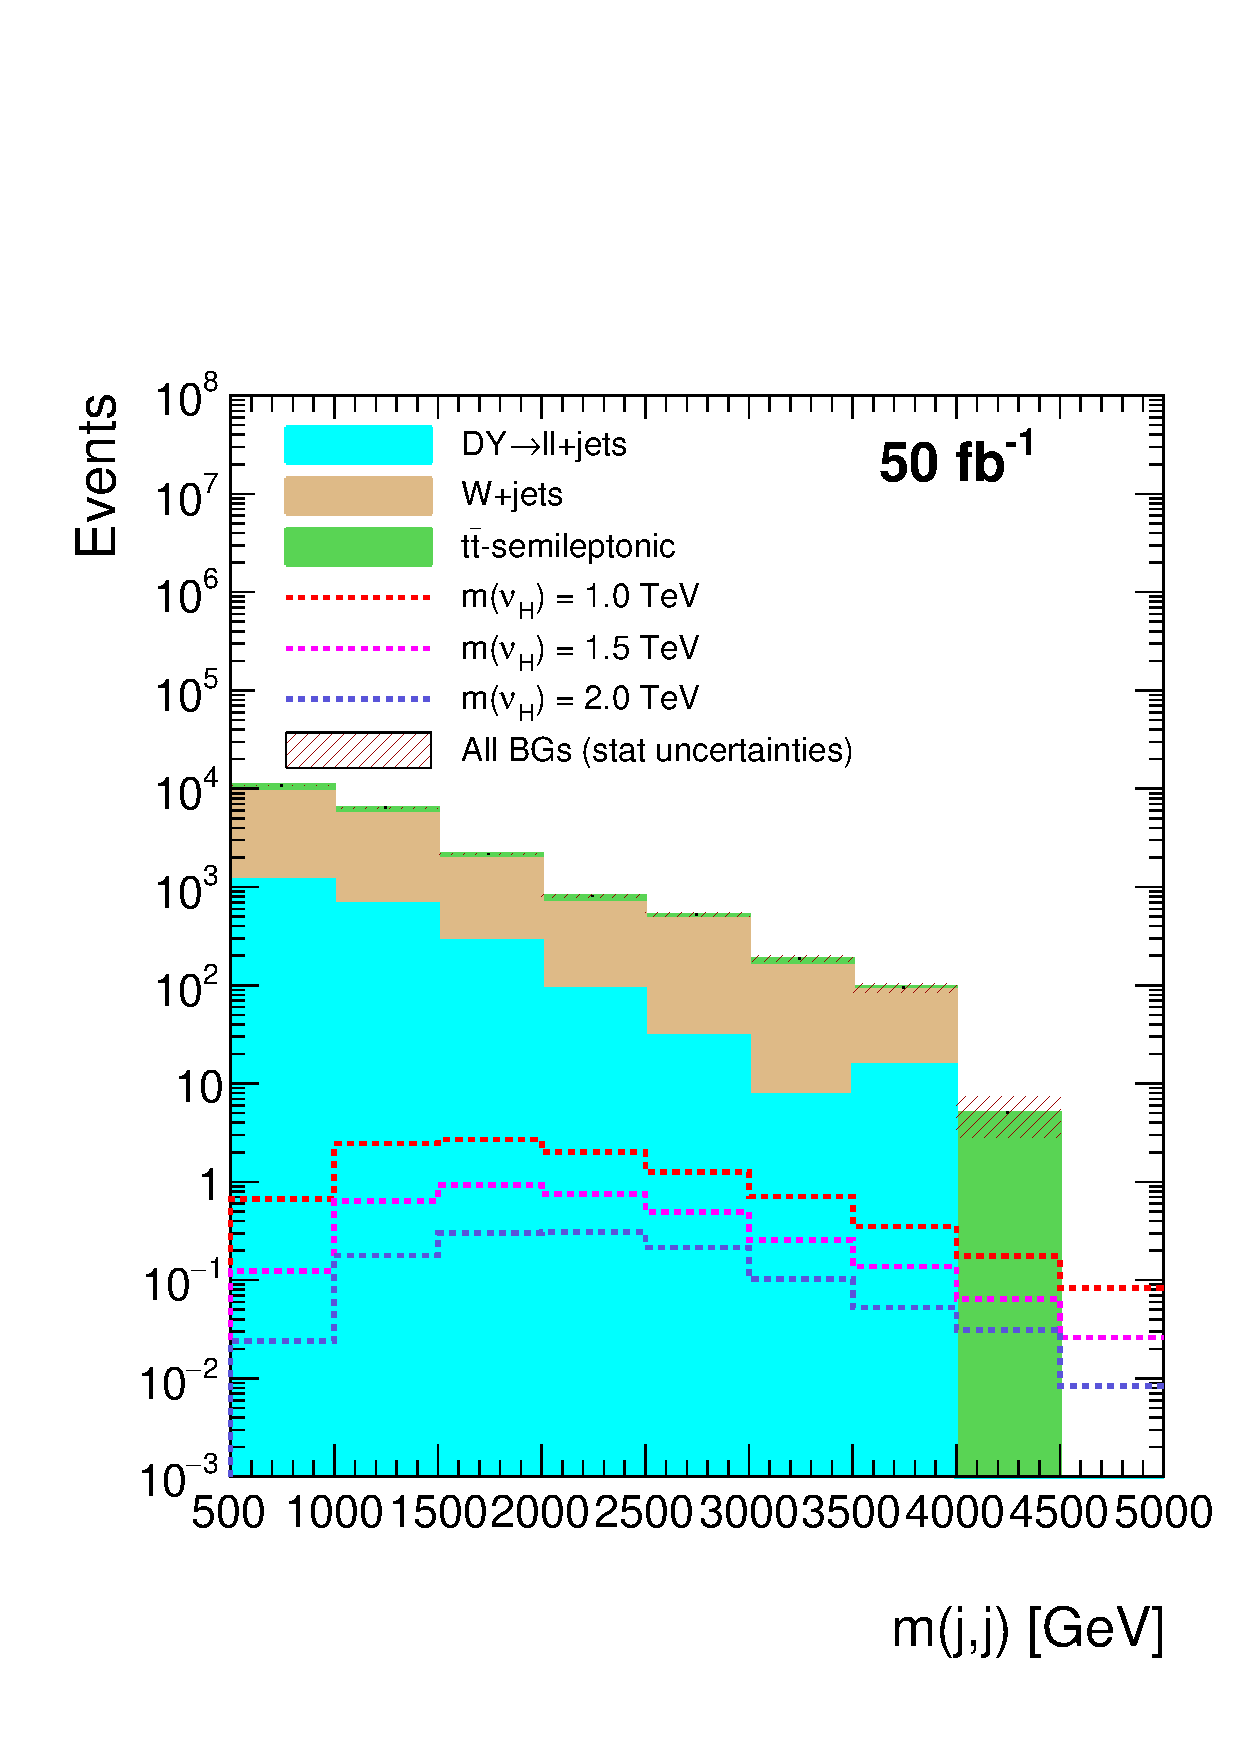
\includegraphics[width=\linewidth]{StackPlots/mjj_1Tau_met60_50ifb.pdf}
\caption{Stack plot of Di-Jet mass requiring only one tau in the event and with $\slashed{E}_{T} > 60$}
\label{fig: mjj1tauMet60}
\end{figure}

\begin{figure}
\centering
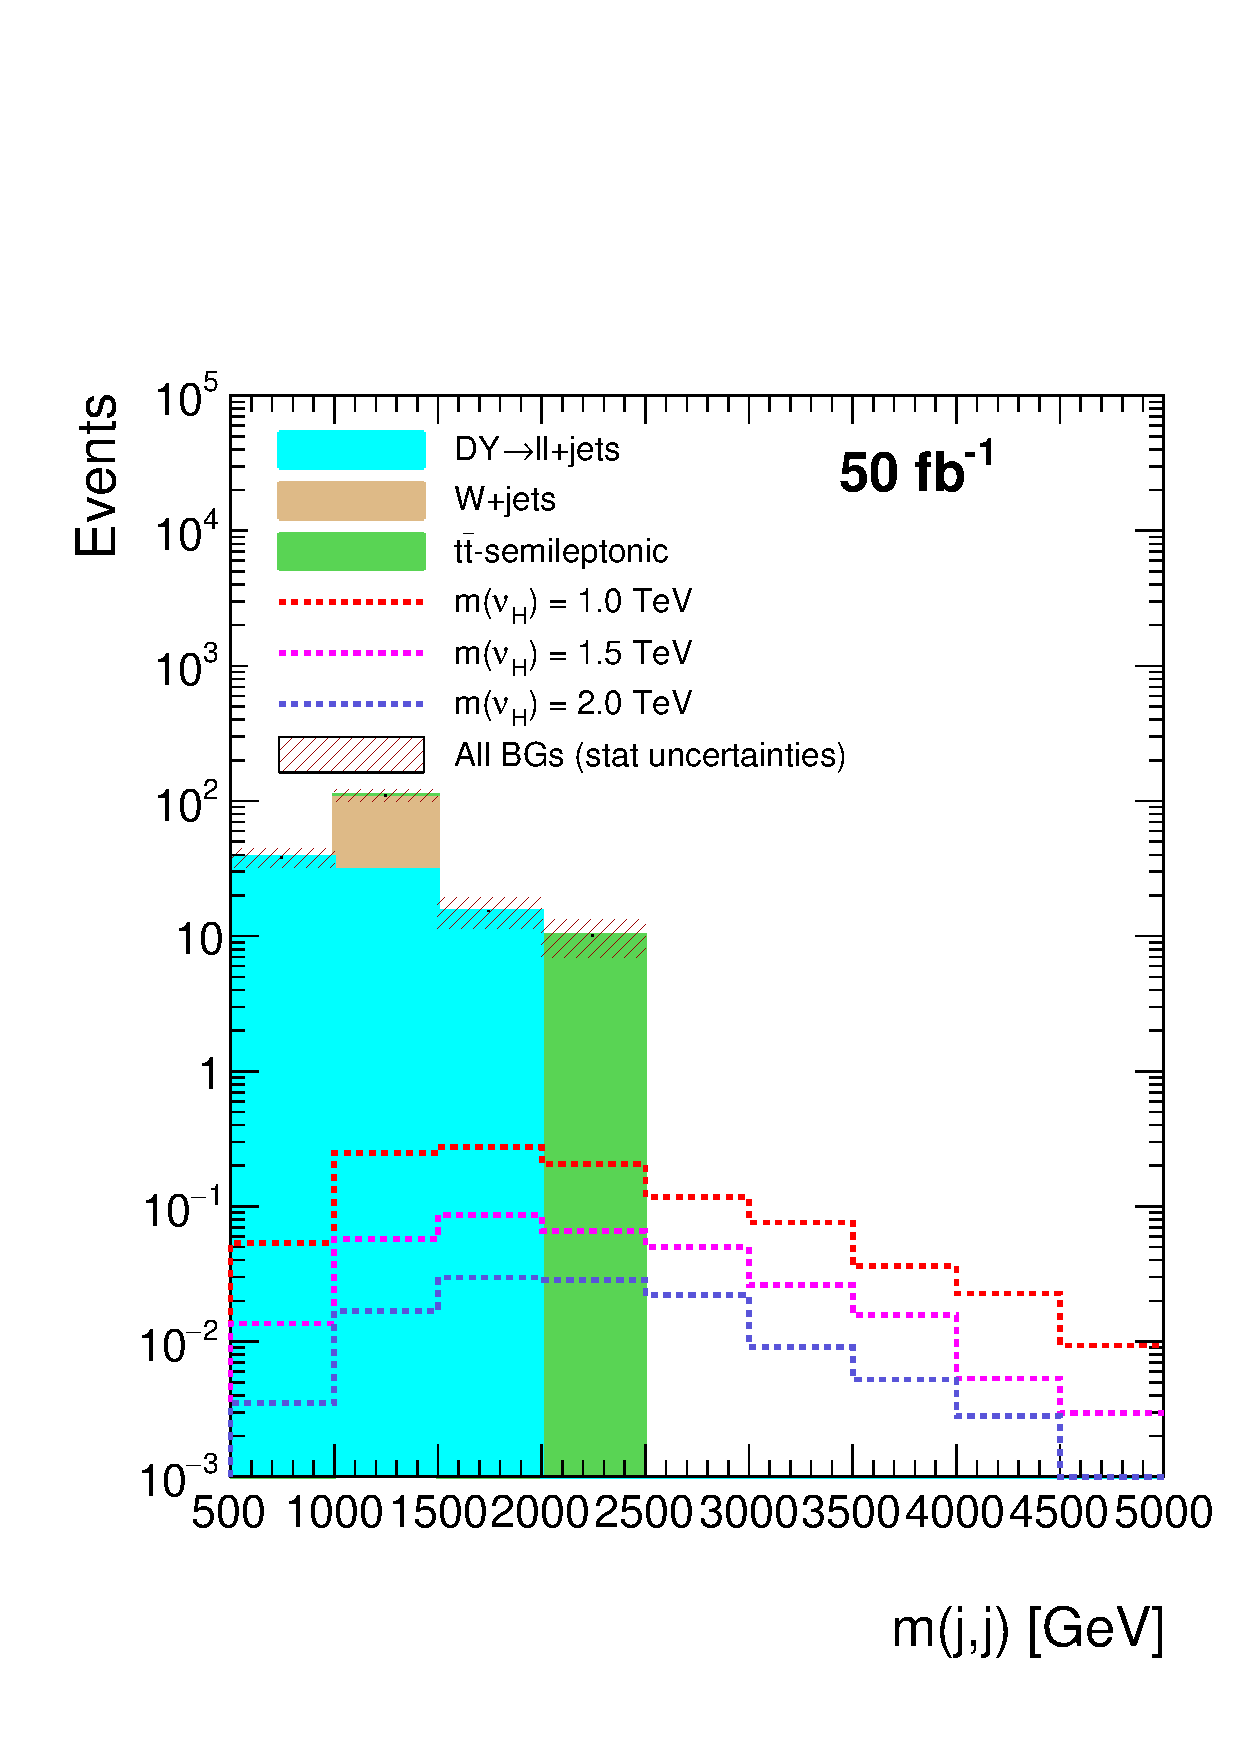
\includegraphics[width=\linewidth]{StackPlots/mjj_2taus_met50_50ifb.pdf}
\caption{Stack plot of Di-Jet mass requiring two taus in the event and with $\slashed{E}_{T} > 50$}
\label{fig: mjj2tauMet50}
\end{figure}

\begin{figure}
\centering
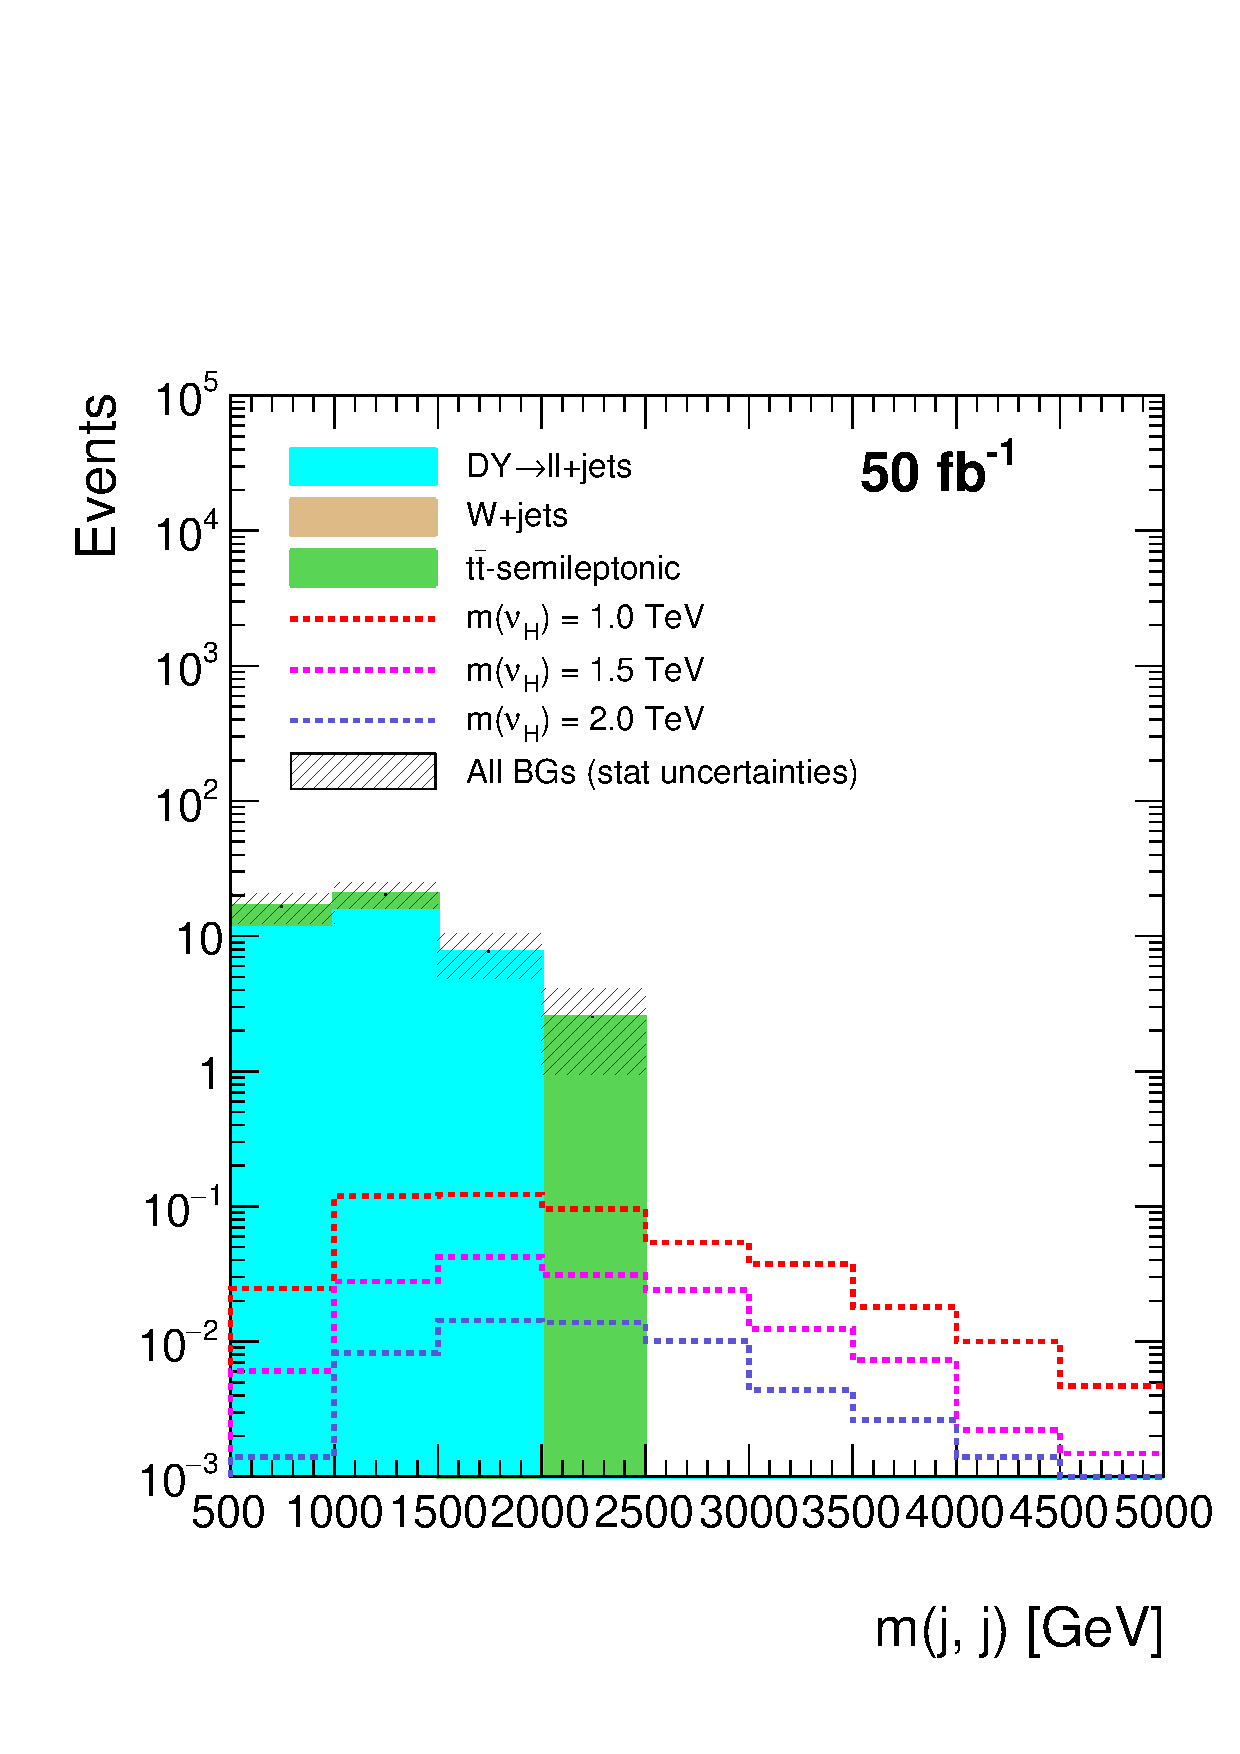
\includegraphics[width=\linewidth]{StackPlots/mjj_2taus_met60_50ifb.pdf}
\caption{Stack plot of Di-Jet mass requiring two taus in the event and with $\slashed{E}_{T} > 60$}
\label{fig: mjj2tauMet60}
\end{figure}

\begin{figure}
\centering
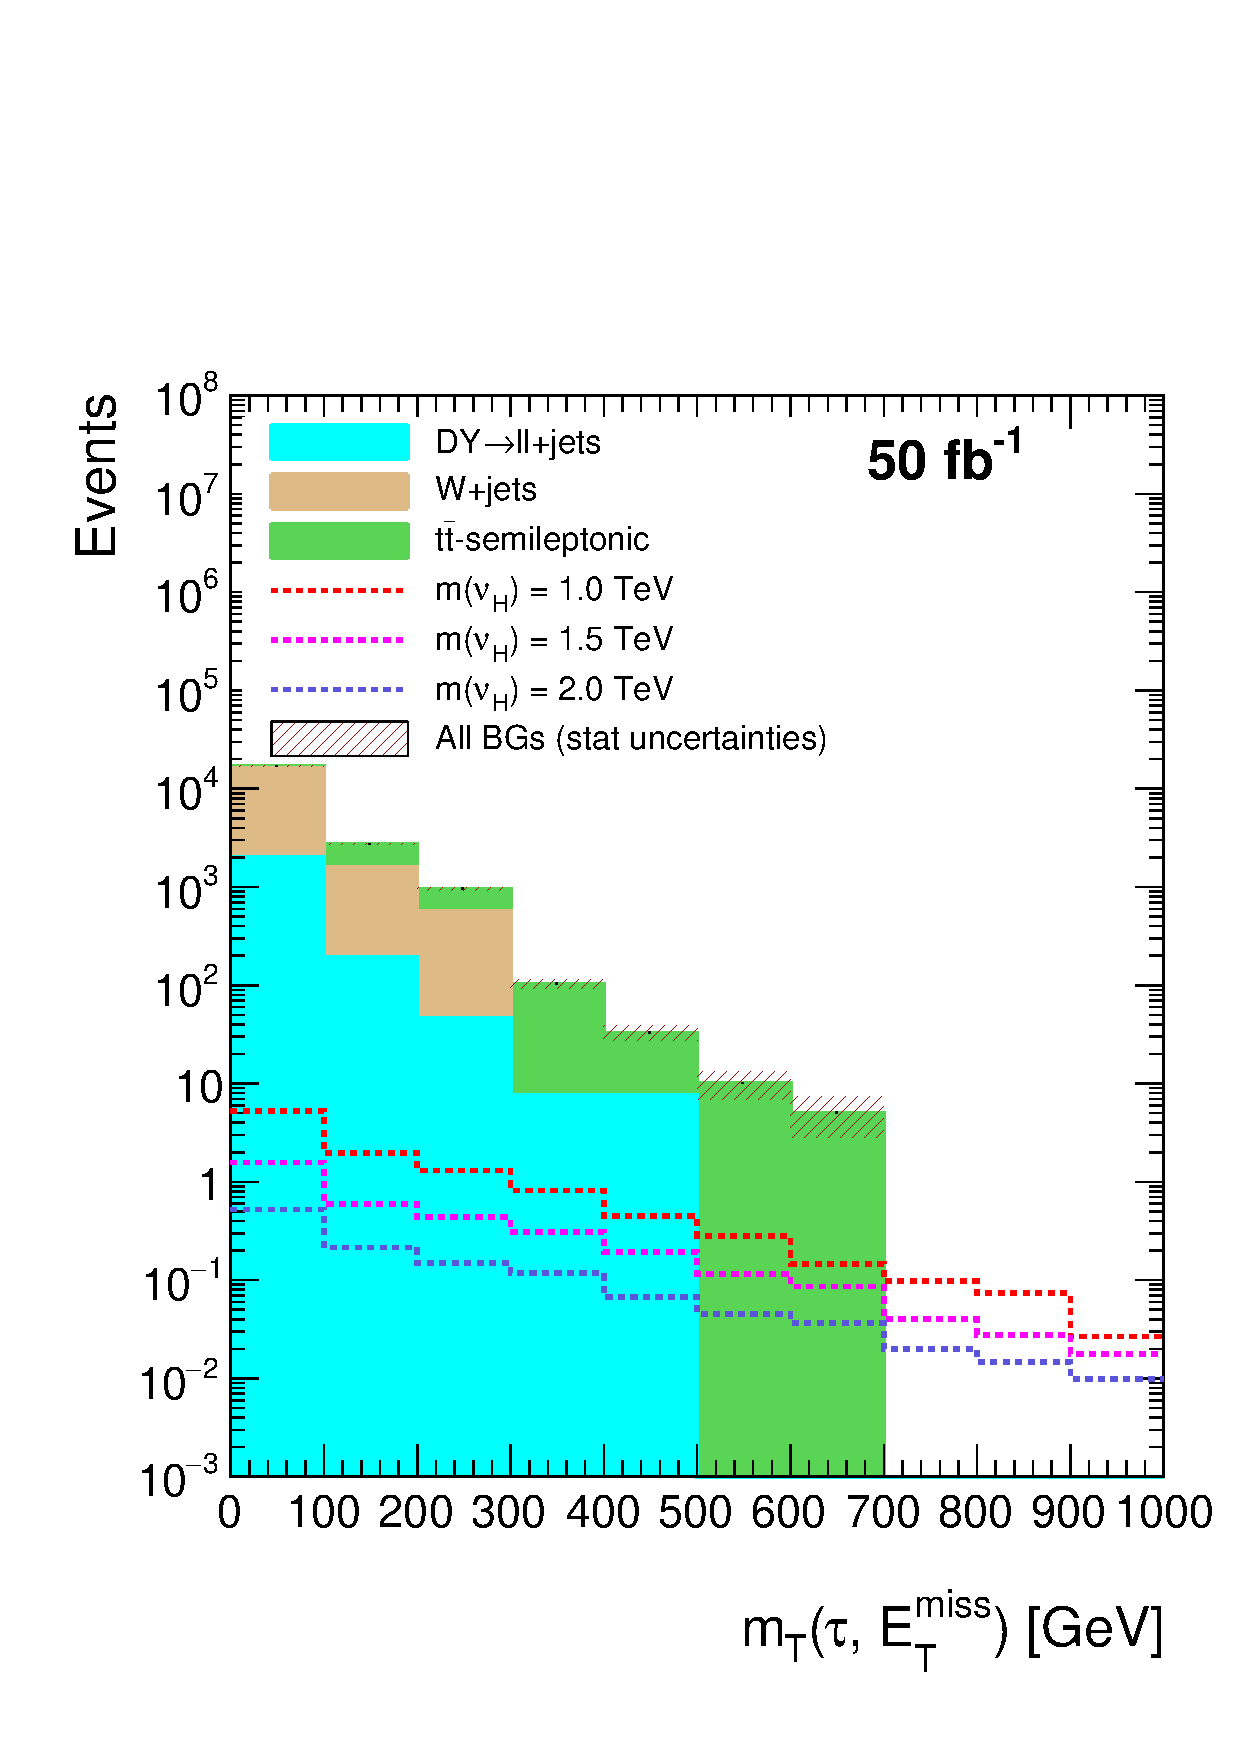
\includegraphics[width=\linewidth]{StackPlots/mT_1Tau_met60_50ifb.pdf}
\caption{Stack plot $m_{T}$ requiring only one tau in the event and with $\slashed{E}_{T} > 60$}
\label{fig: mjj2tauMet50}
\end{figure}

\begin{figure}
\centering
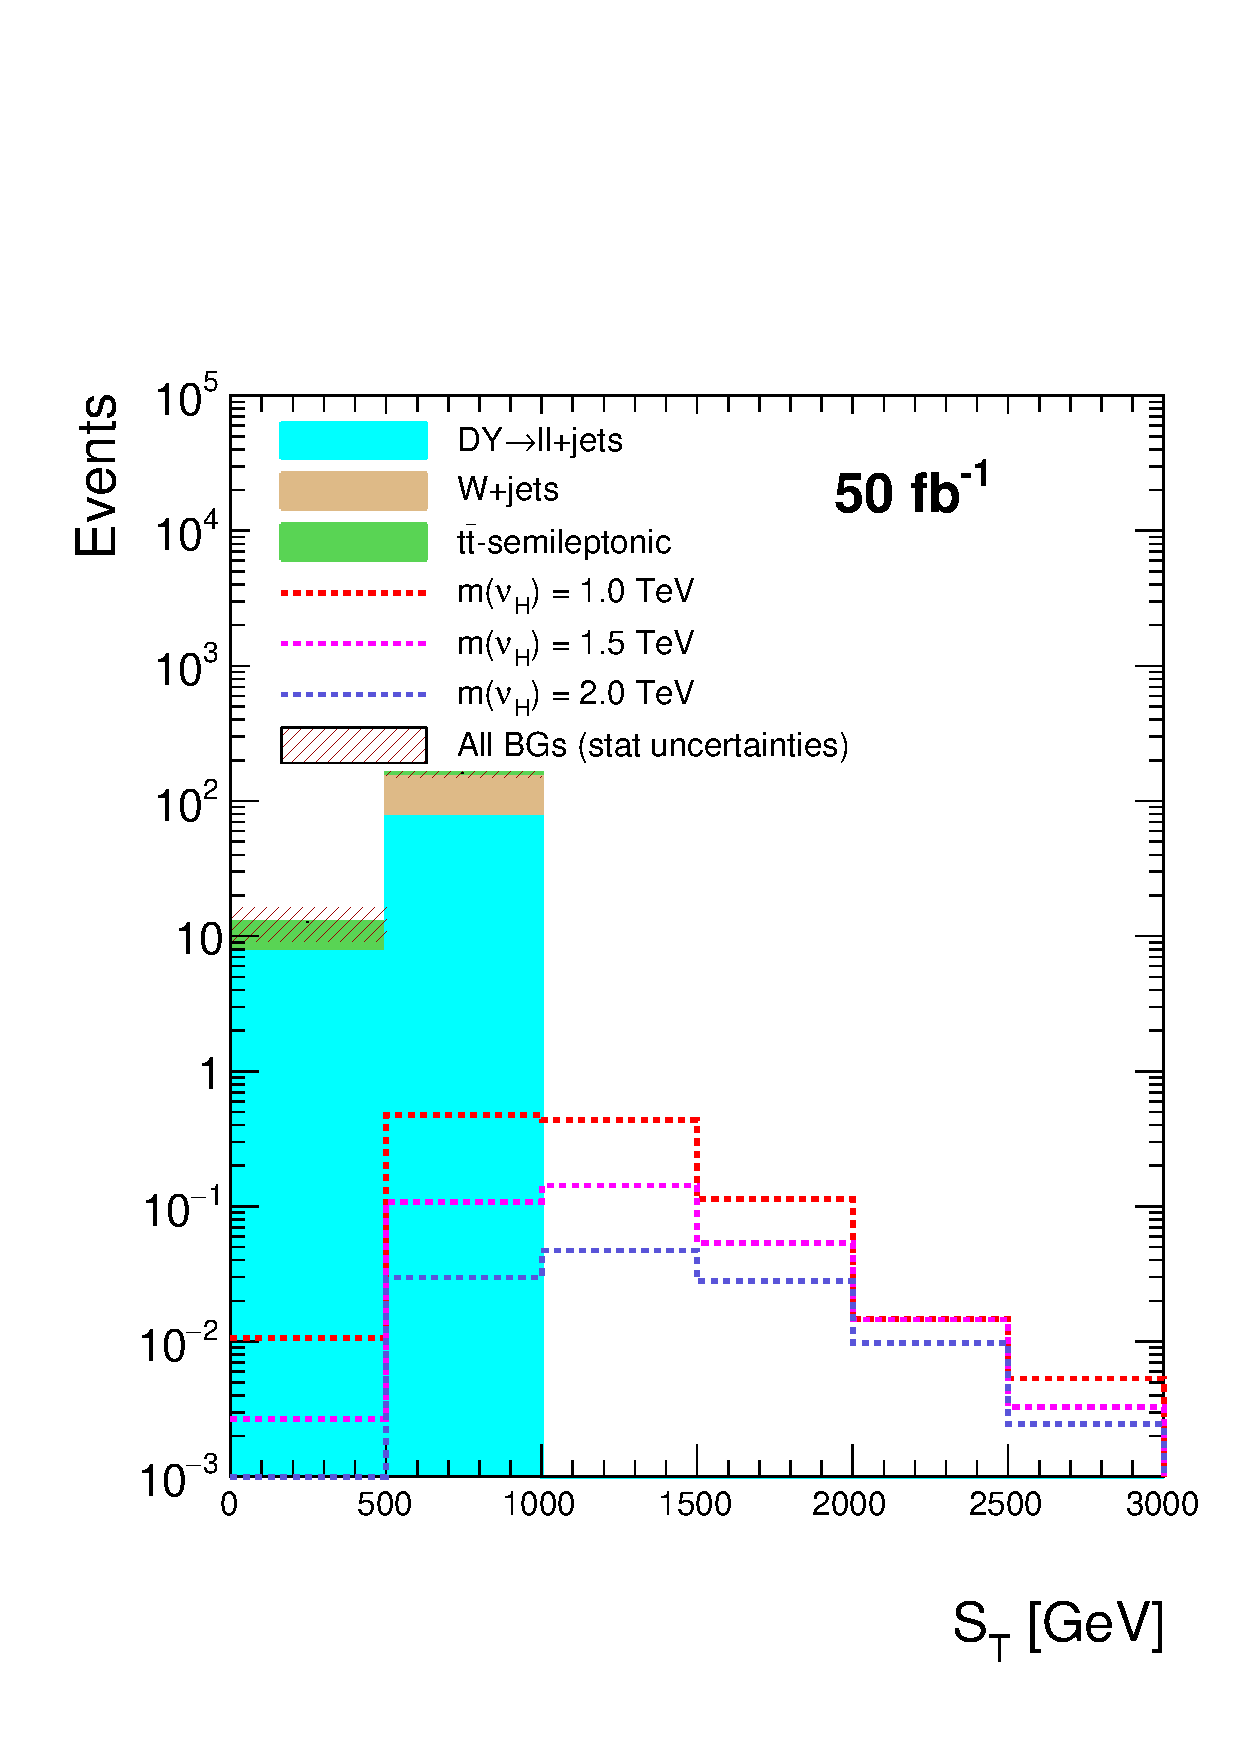
\includegraphics[width=\linewidth]{StackPlots/ST_2taus_met50_50ifb.pdf}
\caption{Stack plot of $S_{T}$ requiring two taus in the event and with $\slashed{E}_{T} > 50$}
\label{fig: HT2tausMet60}
\end{figure}


\begin{figure}
\centering
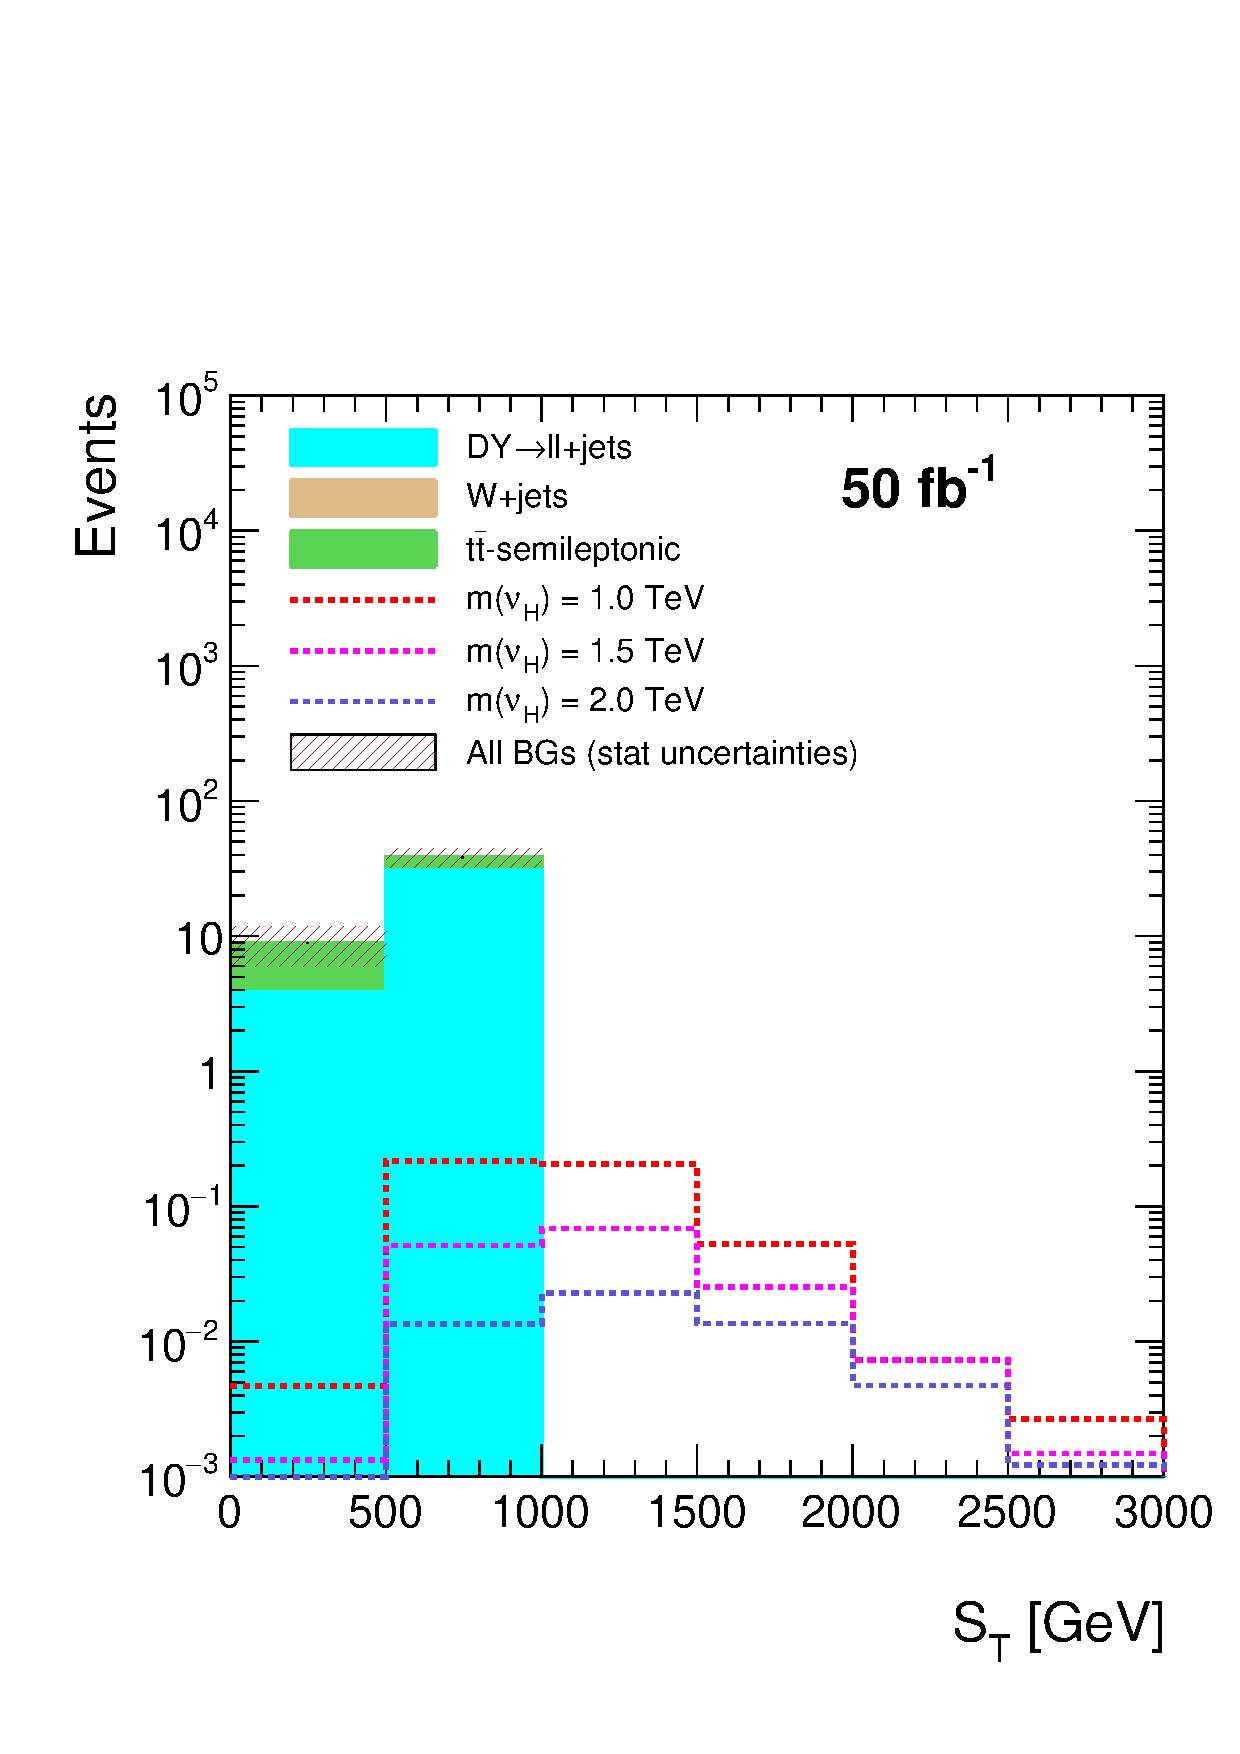
\includegraphics[width=\linewidth]{StackPlots/ST_2taus_met60_50ifb.pdf}
\caption{Stack plot of $S_{T}$ requiring two taus in the event and with $\slashed{E}_{T} > 60$}
\label{fig: HT2tausMet60}
\end{figure}








